\chapter{Sistema multisensorial }
\label{cap:capitulo4}

%\begin{flushright}
%\begin{minipage}[]{10cm}
%\emph{Quizás algún fragmento de libro inspirador...}\\
%\end{minipage}\\

%Autor, \textit{Título}\\
%\end{flushright}

\vspace{1cm}
En este capítulo se describe detalladamente el proceso que se ha llevado a cabo para crear el sistema multisensorial para la monitorización de animales de laboratorio. Como se ha introducido previamente, la aplicación de este trabajo está enfocada a un laboratorio de investigación animal. Concretamente, se ha contactado con el Laboratorio de Bienestar e Investigación Animal de la Universidad de Alcalá de Henares\footnote{\url{https://www.uah.es/es/investigacion/unidades-de-investigacion/grupos-de-investigacion/Bienestar-en-Investigacion-Animal-Welfare-on-Animal-Research./}} para establecer los requisitos software del sistema. Así, el objetivo del trabajo se ha enfocado en la monitorización completa de los ratones del laboratorio, que requieren de una observación constante, así como del entorno en el que se encuentran, debido a que deben estar bajo unas condiciones determinadas.\\

Asimismo, para facilitar la comprensión de los datos por parte de los usuarios finales, se ofrece una interfaz gráfica donde los valores numéricos obtenidos por los sensores, así como cualquier interacción necesaria en la IU (Interfaz de Usuario) se traducen en \textit{widgets} ---pequeñas imágenes que proveen información visual--- comprensibles para cualquier usuario de una manera intuitiva y sencilla. El sistema creado se presenta en la Figura \ref{fig:misistema}.\\
\begin{figure} [h!]
  \begin{center}
    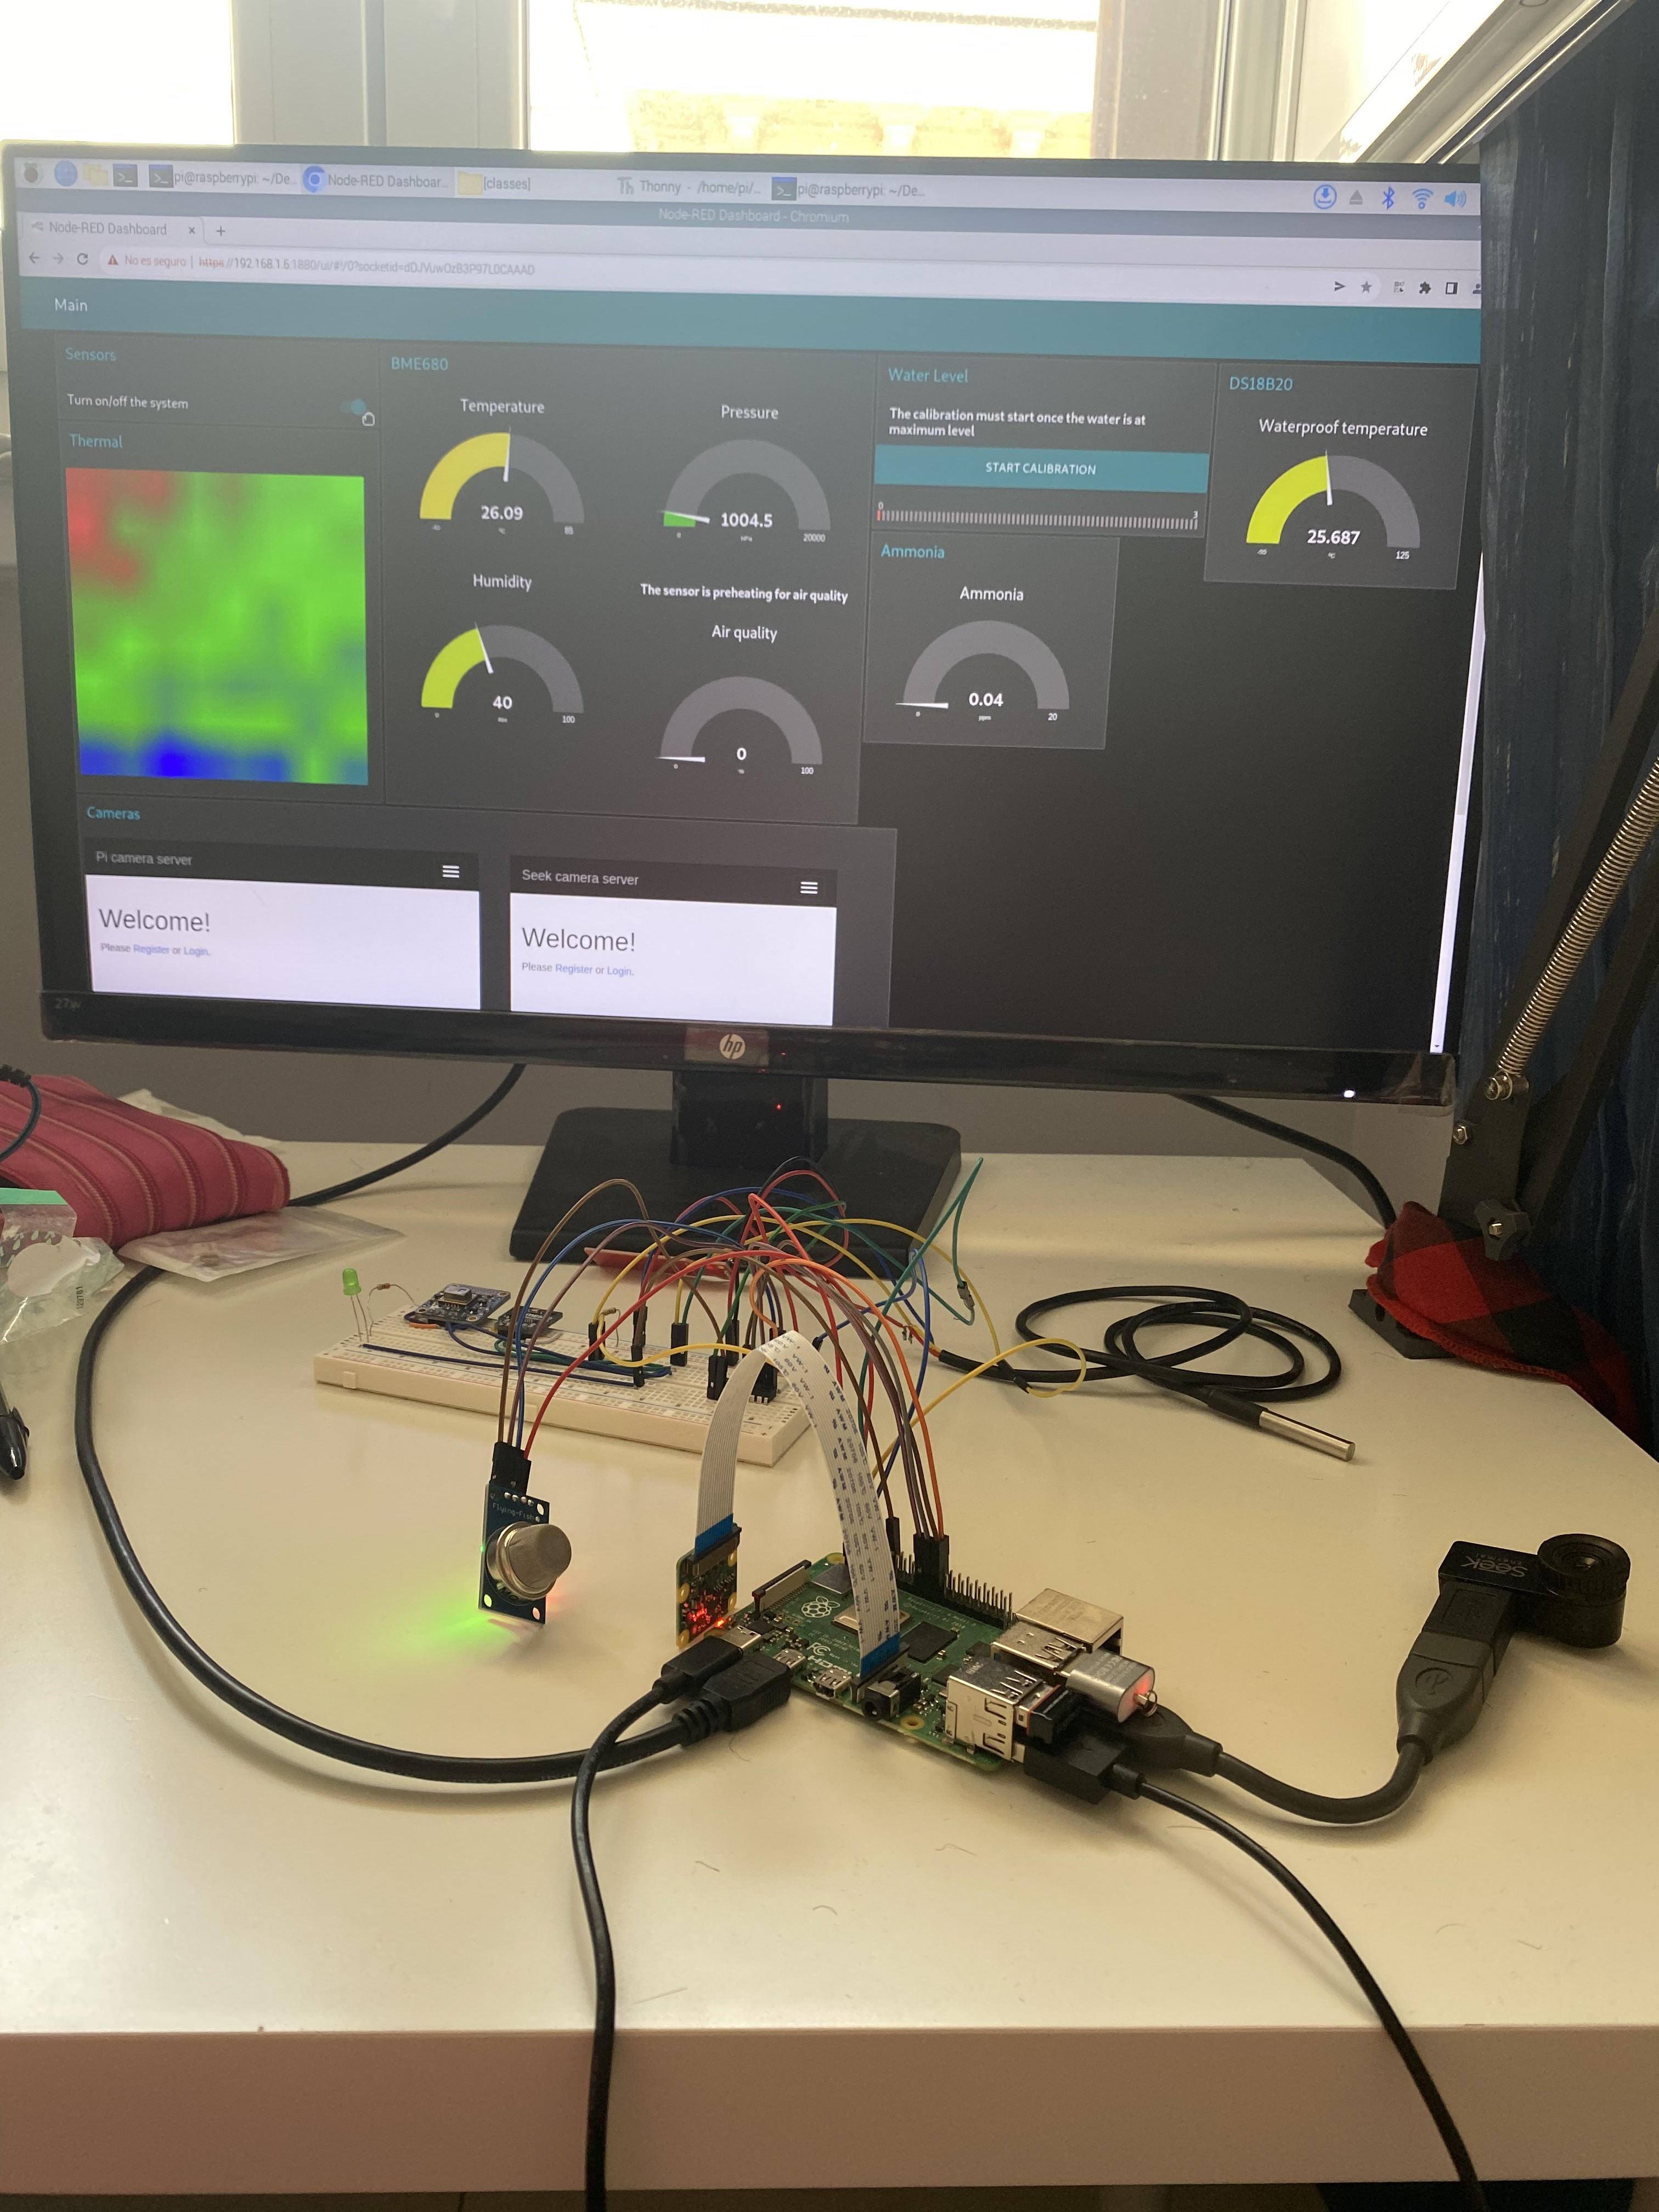
\includegraphics[width=10cm]{figs/misistema}
  \end{center}
  \caption{Sistema resultante.}
  \label{fig:misistema}
\end{figure}

Dos son las partes esenciales para el desarrollo del sistema: hardware y software. En la Sección \ref{sec:deshw} se presenta el desarrollo hardware, y en la Sección \ref{sec:dessw} el desarrollo software que se ha realizado para tener un funcionamiento correcto del sistema.

\section{Desarrollo hardware}
\label{sec:deshw}
La placa que se ha utilizado para el proyecto es la Raspberry Pi 4B (Figura \ref{fig:rasp}-a), el último modelo de Raspberry y muy utilizada para el desarrollo de proyectos debido ---entre otras cosas--- a su bajo coste. Este modelo es el más rápido y potente, ofreciendo de dos a tres veces el rendimiento del procesador de su modelo predecesor, la Raspberry Pi 3b+. El sistema operativo utilizado para el desarrollo del proyecto ha sido Raspbian (Figura \ref{fig:rasp}-b), sobre la versión de 64 bits.\\
\begin{figure}[h!]
  \begin{center}
    \subfigure[Raspberry Pi 4B utilizada para el desarrollo del presente TFG.]{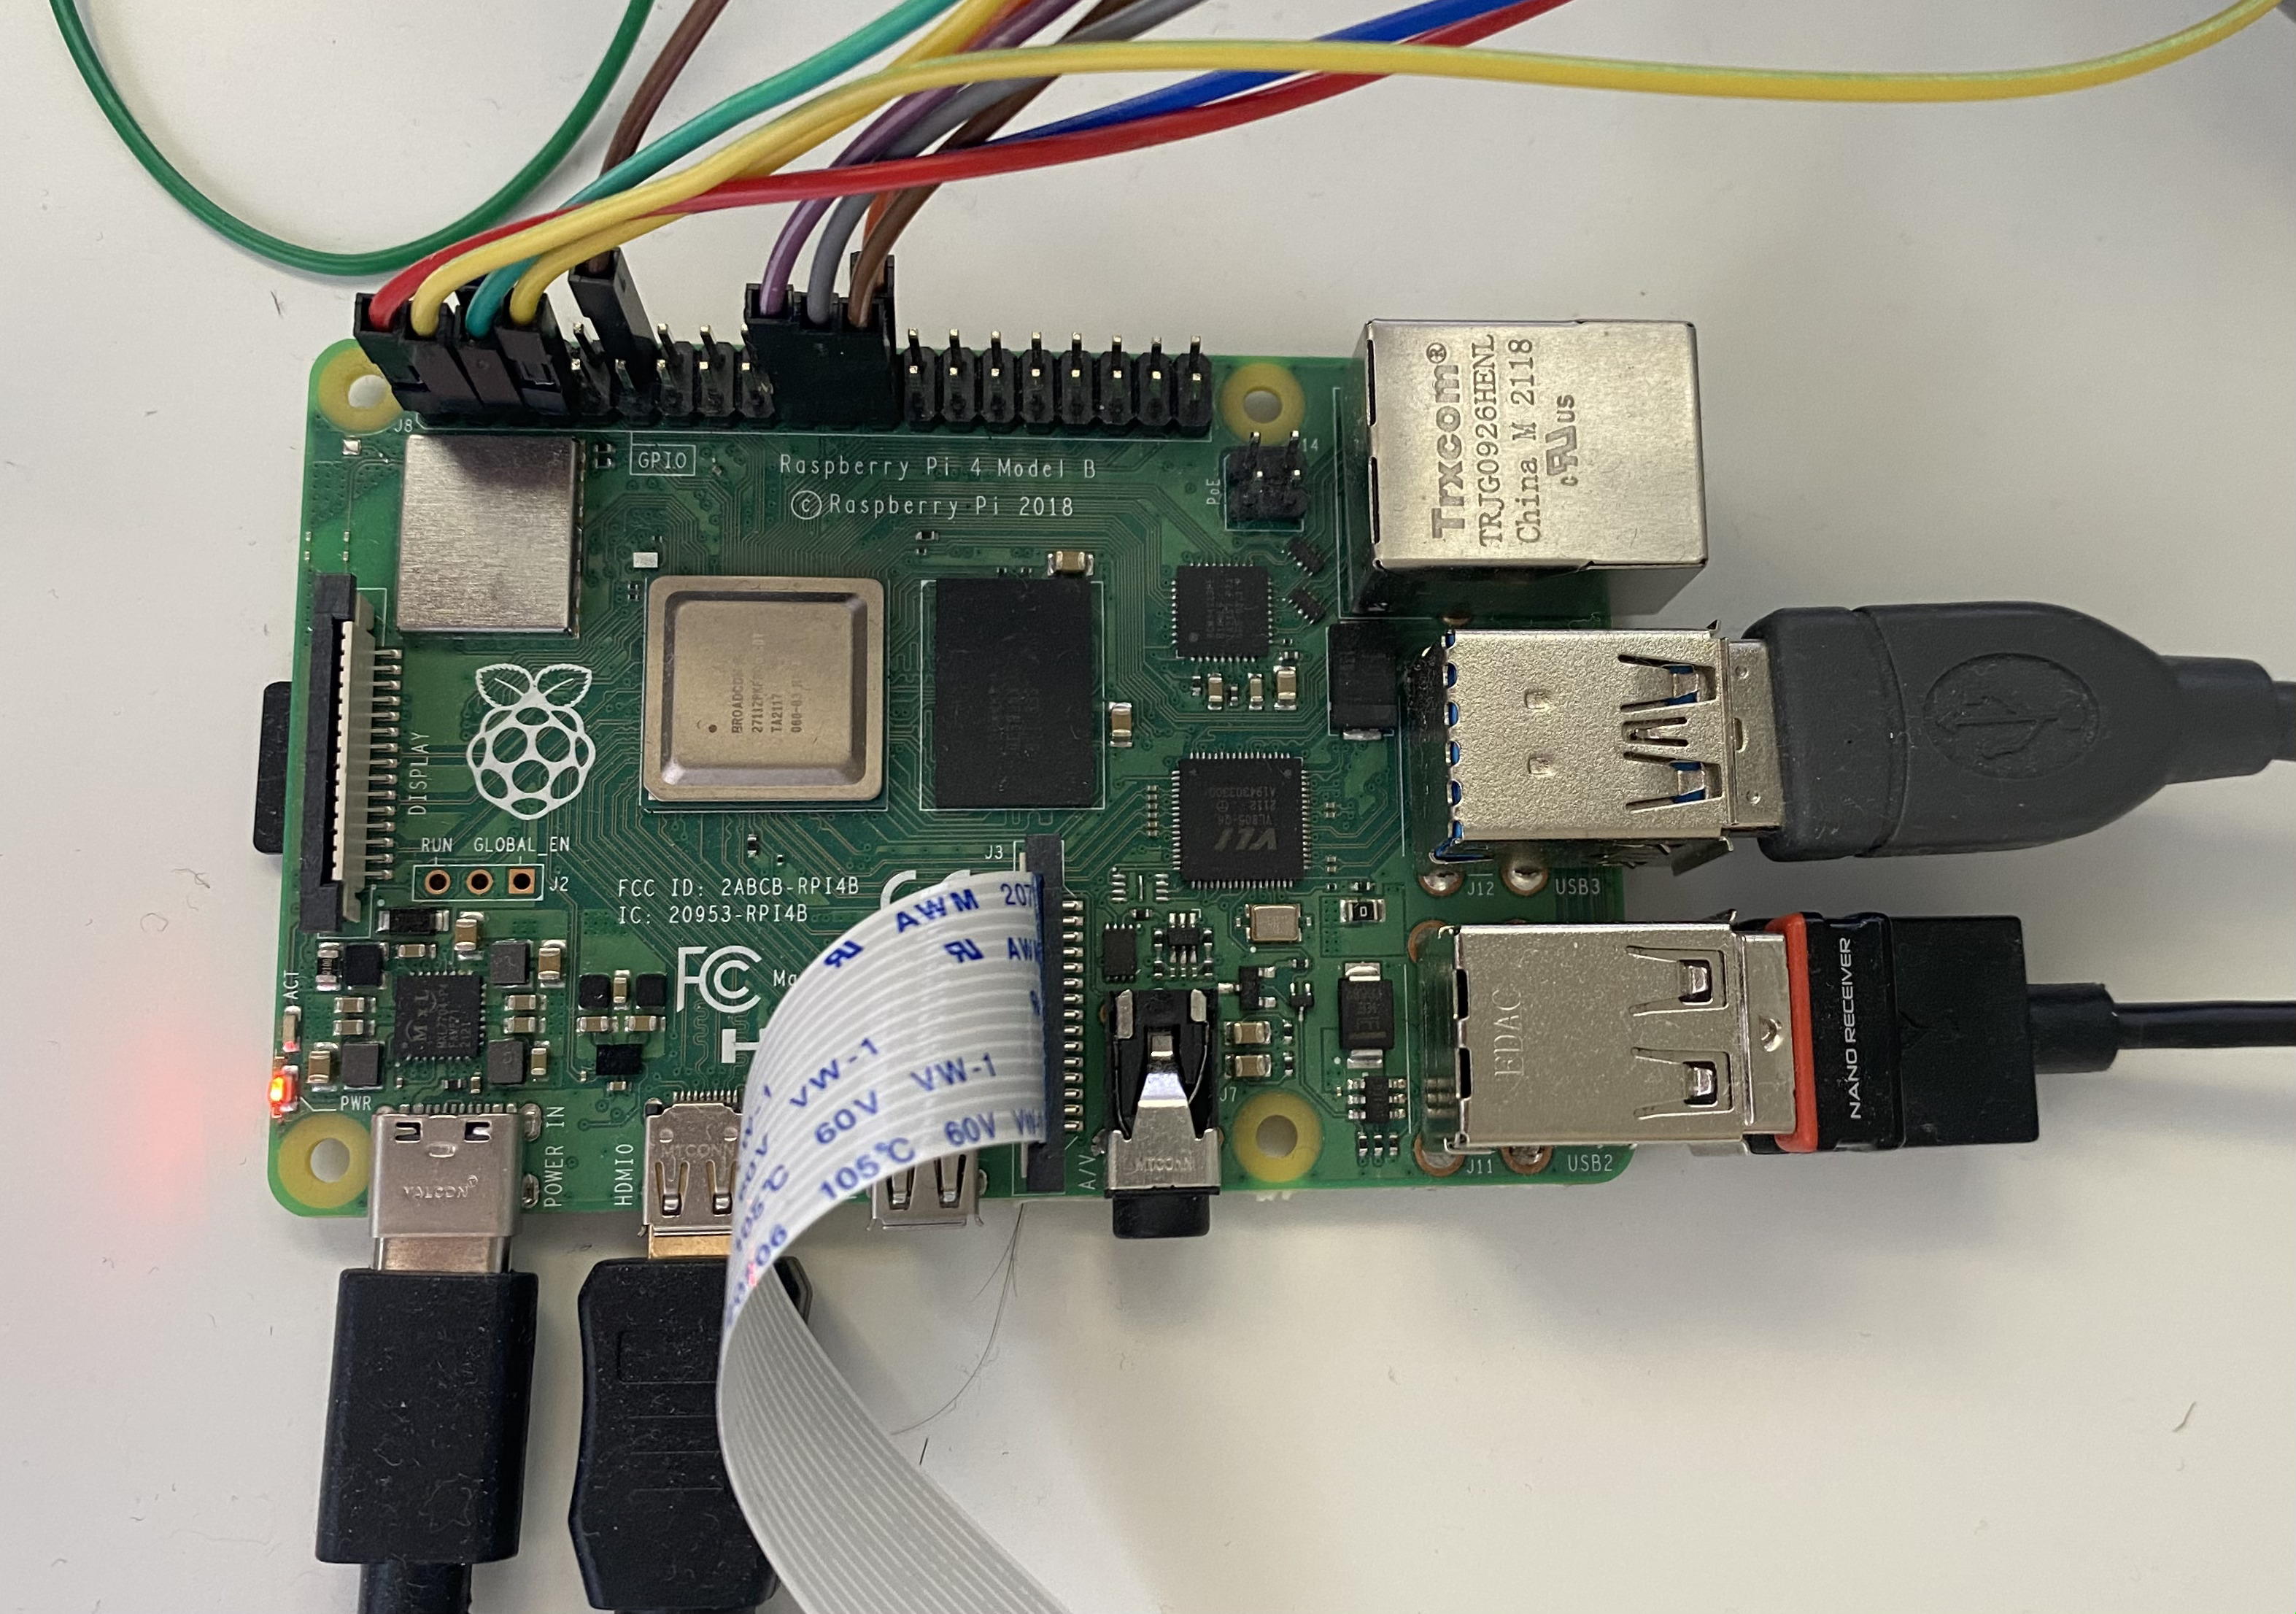
\includegraphics[width=12cm]{figs/raspberry}}\hspace{1mm}
    \subfigure[Entorno de trabajo en Raspbian.]{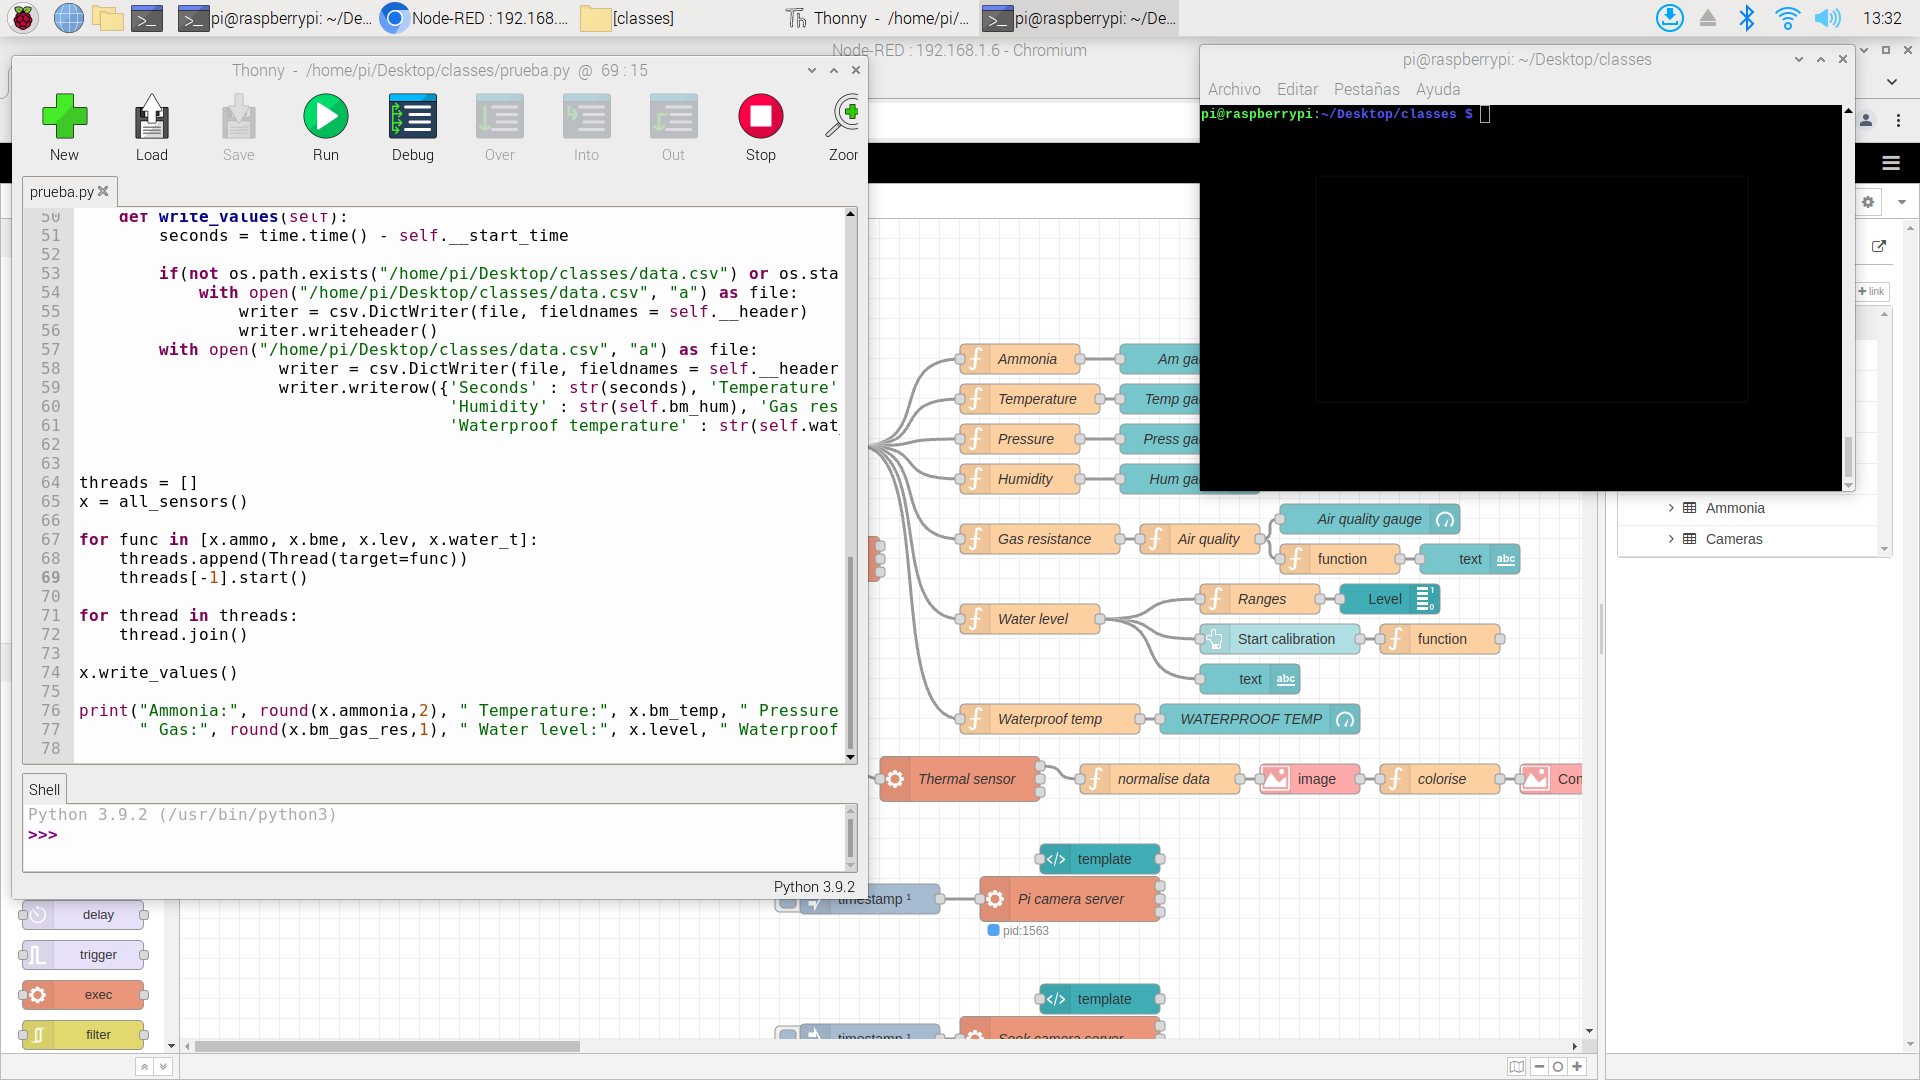
\includegraphics[width=12cm]{figs/trabajo}}
  \end{center}
\caption{Imágenes del HW y SW usados para el TFG.} \label{fig:rasp}
\end{figure}

Se han utilizado los puertos GPIO para la conexión de los distintos sensores presentados en la Sección \ref{sec:hw}. En la Figura \ref{fig:esquema} se encuentran las distintas conexiones de los sensores a la Raspberry.\\
\begin{figure} [h!]
  \begin{center}
    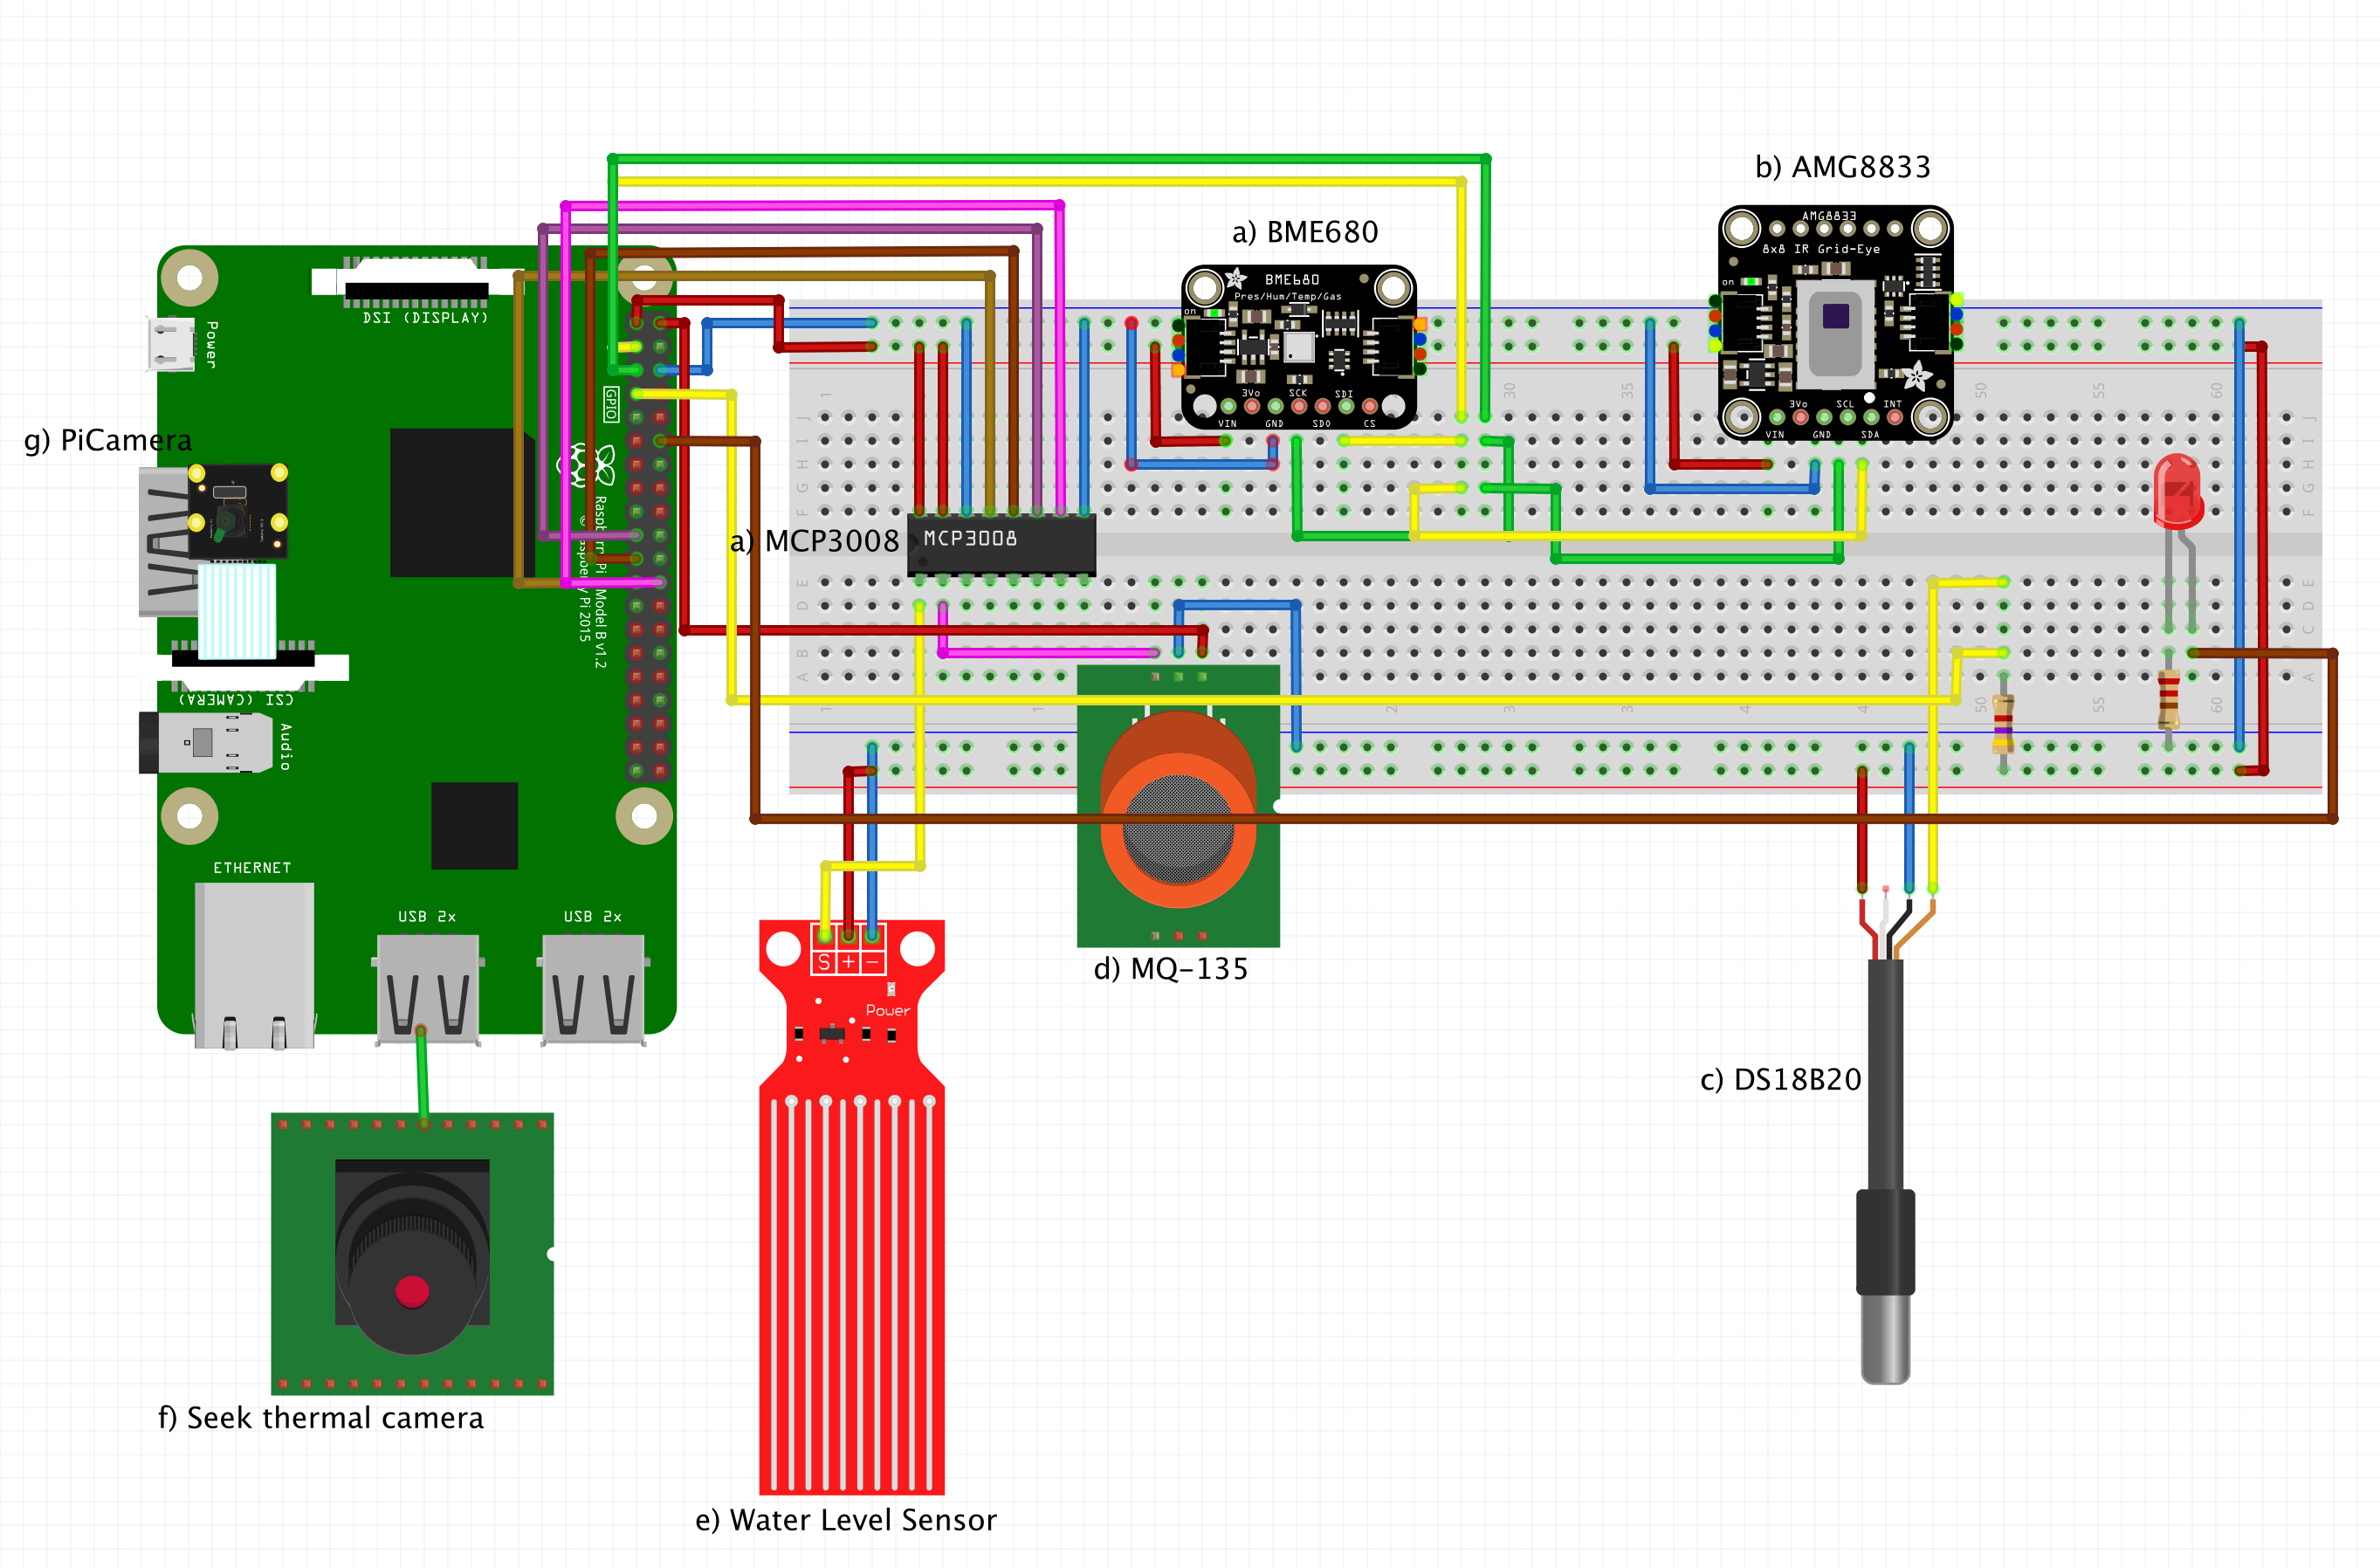
\includegraphics[width=14cm]{figs/esquema}
  \end{center}
  \caption{Esquema de conexiones.}
  \label{fig:esquema}
\end{figure}

A continuación se explican con más detalle la conexión de estos sensores:
\begin{itemize}
\item{Sensor BME680 (Figura \ref{fig:bme_of}).} Este sensor funciona con conexión I2C, que para su funcionamiento necesita dos pines; SDA y SCL. Por tanto, siguiendo el esquema de la Figura \ref{fig:pinout}, se ha conectado a los pines 3 y 5. También se ha conectado al pin 1 para obtener la alimentación de 3.3V que necesita y al pin 6 (a tierra), para evitar que se rompa el sensor.

\item{Sensor AMG8833 (Figura \ref{fig:termicos}-a).} Este sensor también funciona con conexión I2C. Por tanto su conexión es igual al sensor anterior: Conexión a los pines 3 y 5 para la conexión I2C y a los pines 1 y 6 para la alimentación y tierra, respectivamente. En la Figura \ref{fig:esquema}, la conexión a alimentación viene representada con el cable rojo, la conexión a tierra con el cable azul, la conexión I2C al pin SDA con el cable amarillo y la conexión I2C al pin SCL con el cable verde.

\item{Sensor DS18B20 (Figura \ref{fig:ds_of}).} Este sensor necesita ser conectado con una resistencia de 4.7K $\Omega$ para mantener los datos estables. Su conexión por tanto es a los pines 1 y 6 para alimentación a 3.3V y tierra, y al pin 7 para la obtención de las medidas, tal y como aparece en el esquema de la Figura \ref{fig:esquema}. 

\item{MQ-135 (Figura \ref{fig:mq_of}).} Este sensor necesita ser conectado a un conversor analógico a digital debido a que se deben obtener medidas analógicas. Como aparece en la Figura \ref{fig:esquema}, se ha utilizado el conversor MCP3008. Además, se ha conectado a los pines 2 para la alimentación de 5V que necesita y 6 para la conexión a tierra.

\item{Sensor nivel de agua (Figura \ref{fig:nivel_of}).} Igual que el sensor anterior, este también necesita lecturas analógicas, por lo que se ha conectado al conversor, al pin 1 para la alimentación de 3.3V y al 6 para la conexión a tierra.

\item{Seek thermal (Figura \ref{fig:termicos}-b).} Este sensor se ha conectado a través de una de las entradas USB que dispone Raspberry usando un conversor de USB a micro USB.

\item{PiCamera (Figura \ref{fig:picam_of}).} Este sensor se ha conectado en el puerto J3 que ofrece Raspberry para la conexión de su cámara. 
\end{itemize}

\section{Desarrollo software}
\label{sec:dessw}
Tras diseñar la plataforma hardware, el siguiente paso es darle el soporte software. Y es que, para que este sistema funcione, es necesario crear las instrucciones y reglas a través de programas o aplicaciones, esto es, la parte software.\\

El primer, y más importante paso en cualquier desarrollo software es establecer los requisitos del sistema. Para ello, y como se ha comentado previamente, se han mantenido reuniones con el Laboratorio de Bienestar e Investigación Animal de la Universidad de Alcalá de Henares, así como reuniones semanales con el tutor. De estas reuniones se ha obtenido la información necesaria para poder hacer el diseño software del sistema, que queda reflejado mediante el diagrama de casos de uso (Figura \ref{fig:casos}) y, tras un análisis de este, el diagrama de clases (Figura \ref{fig:umlet}).\\
\begin{figure} [h!]
  \begin{center}
    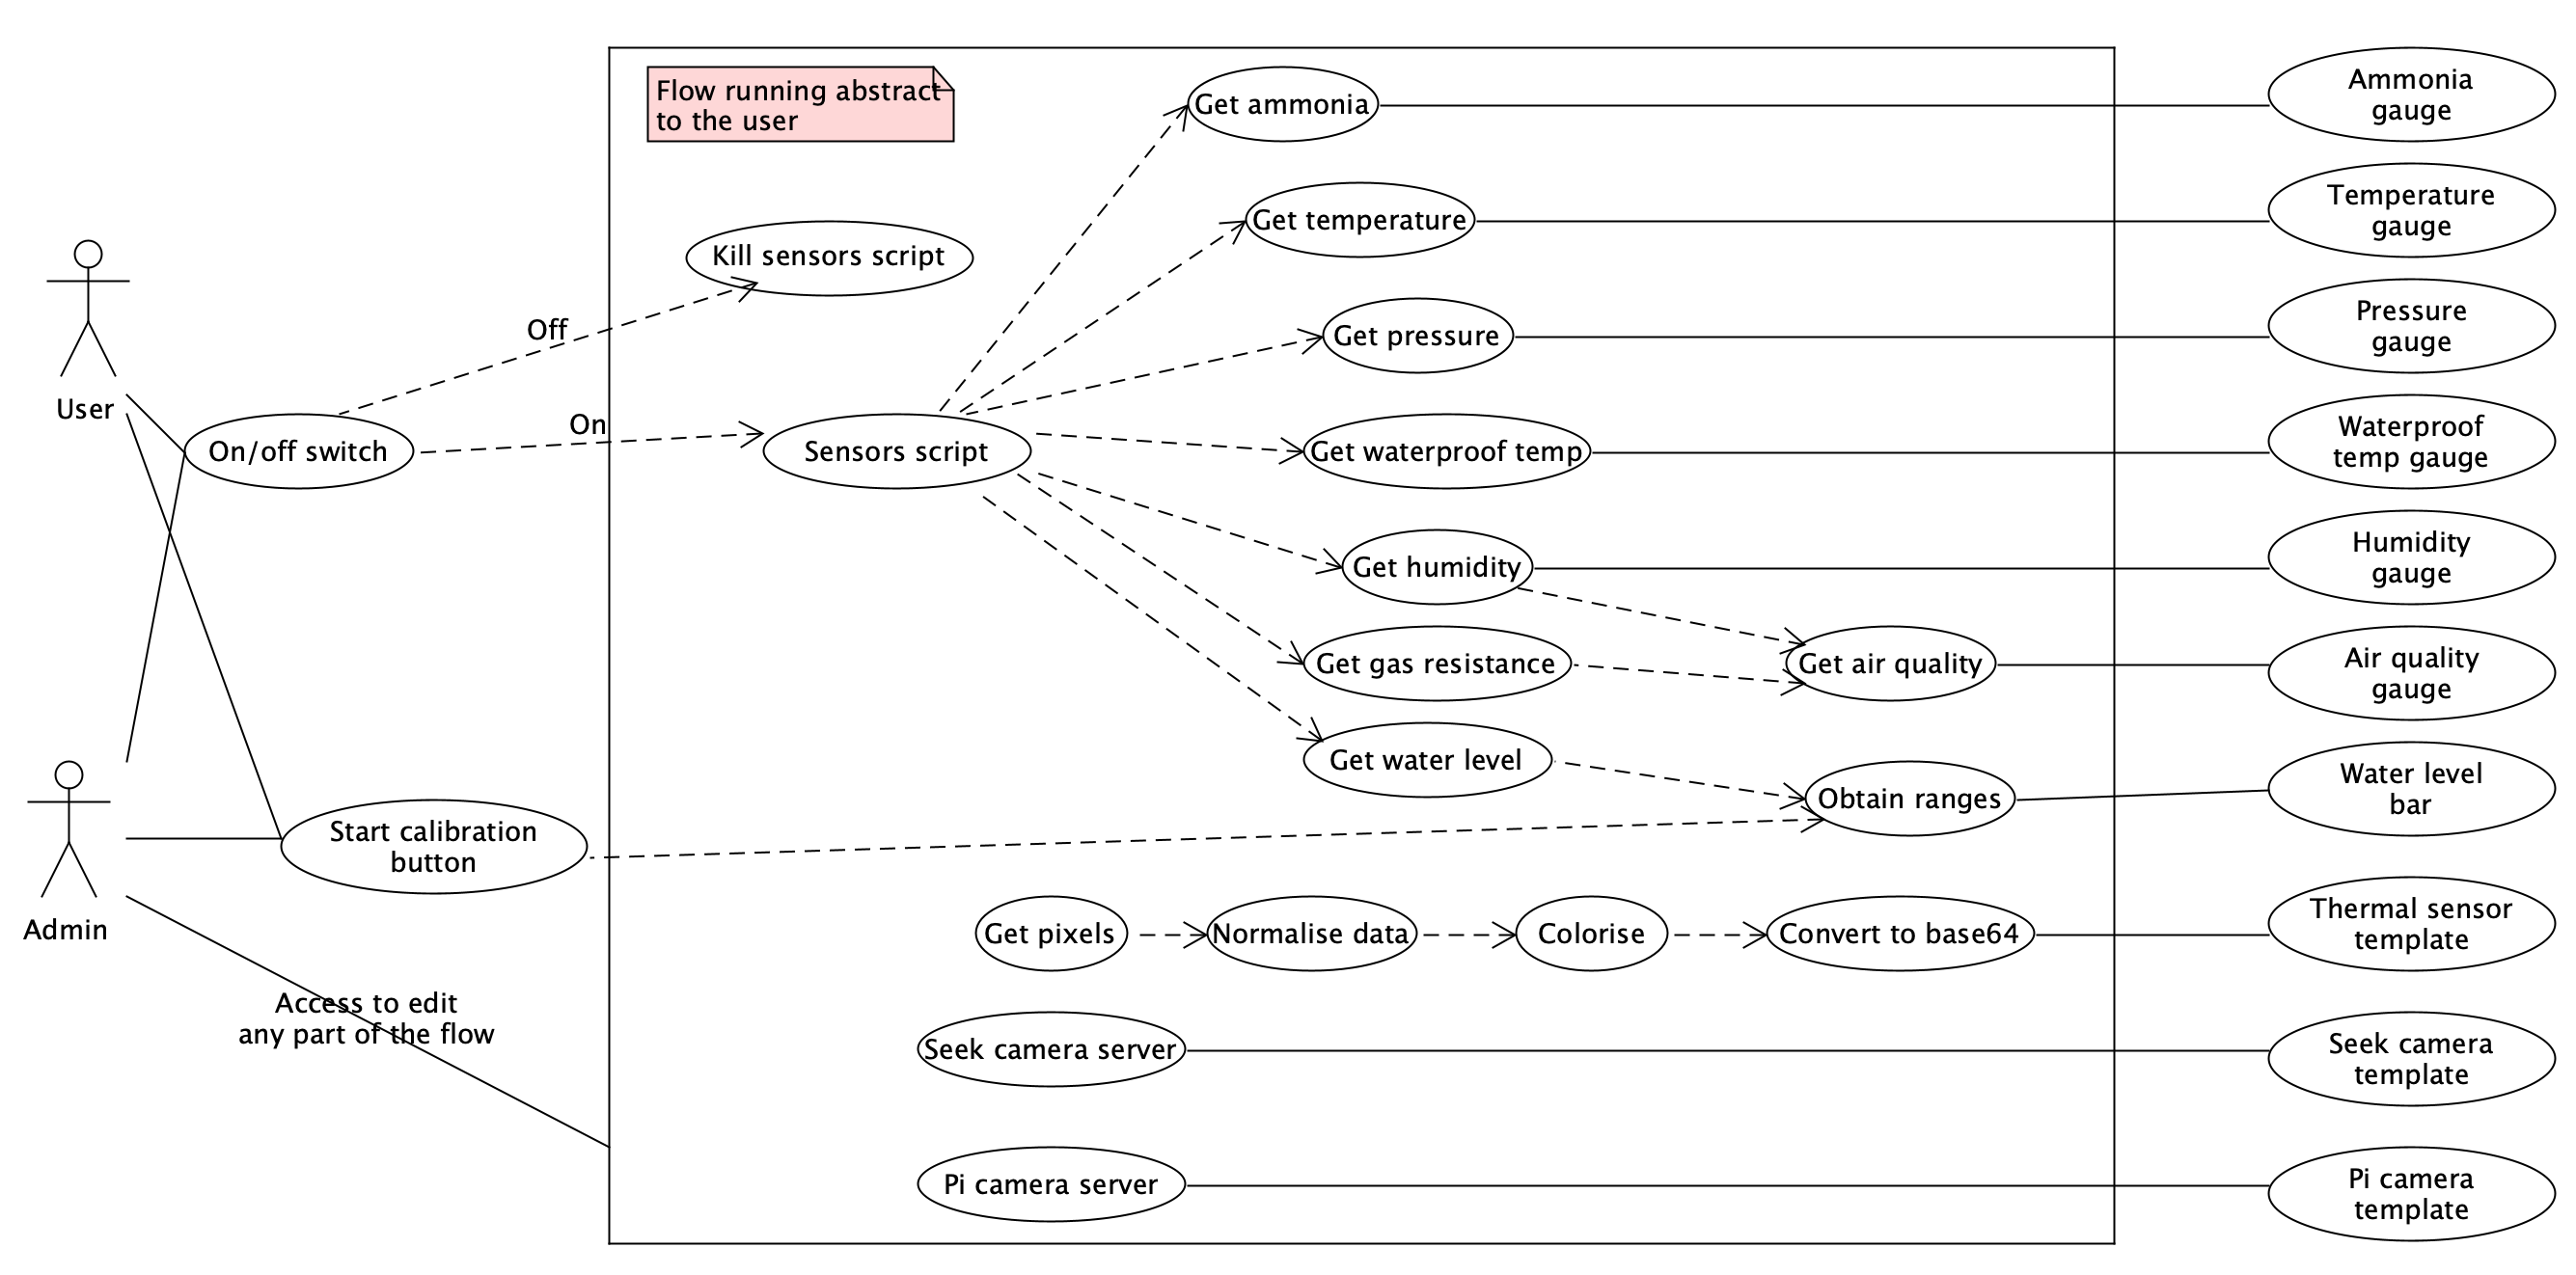
\includegraphics[width=17cm]{figs/casos}
  \end{center}
  \caption{Diagrama de casos de uso del sistema.}
  \label{fig:casos}
\end{figure}

\begin{figure} [h!]
  \begin{center}
    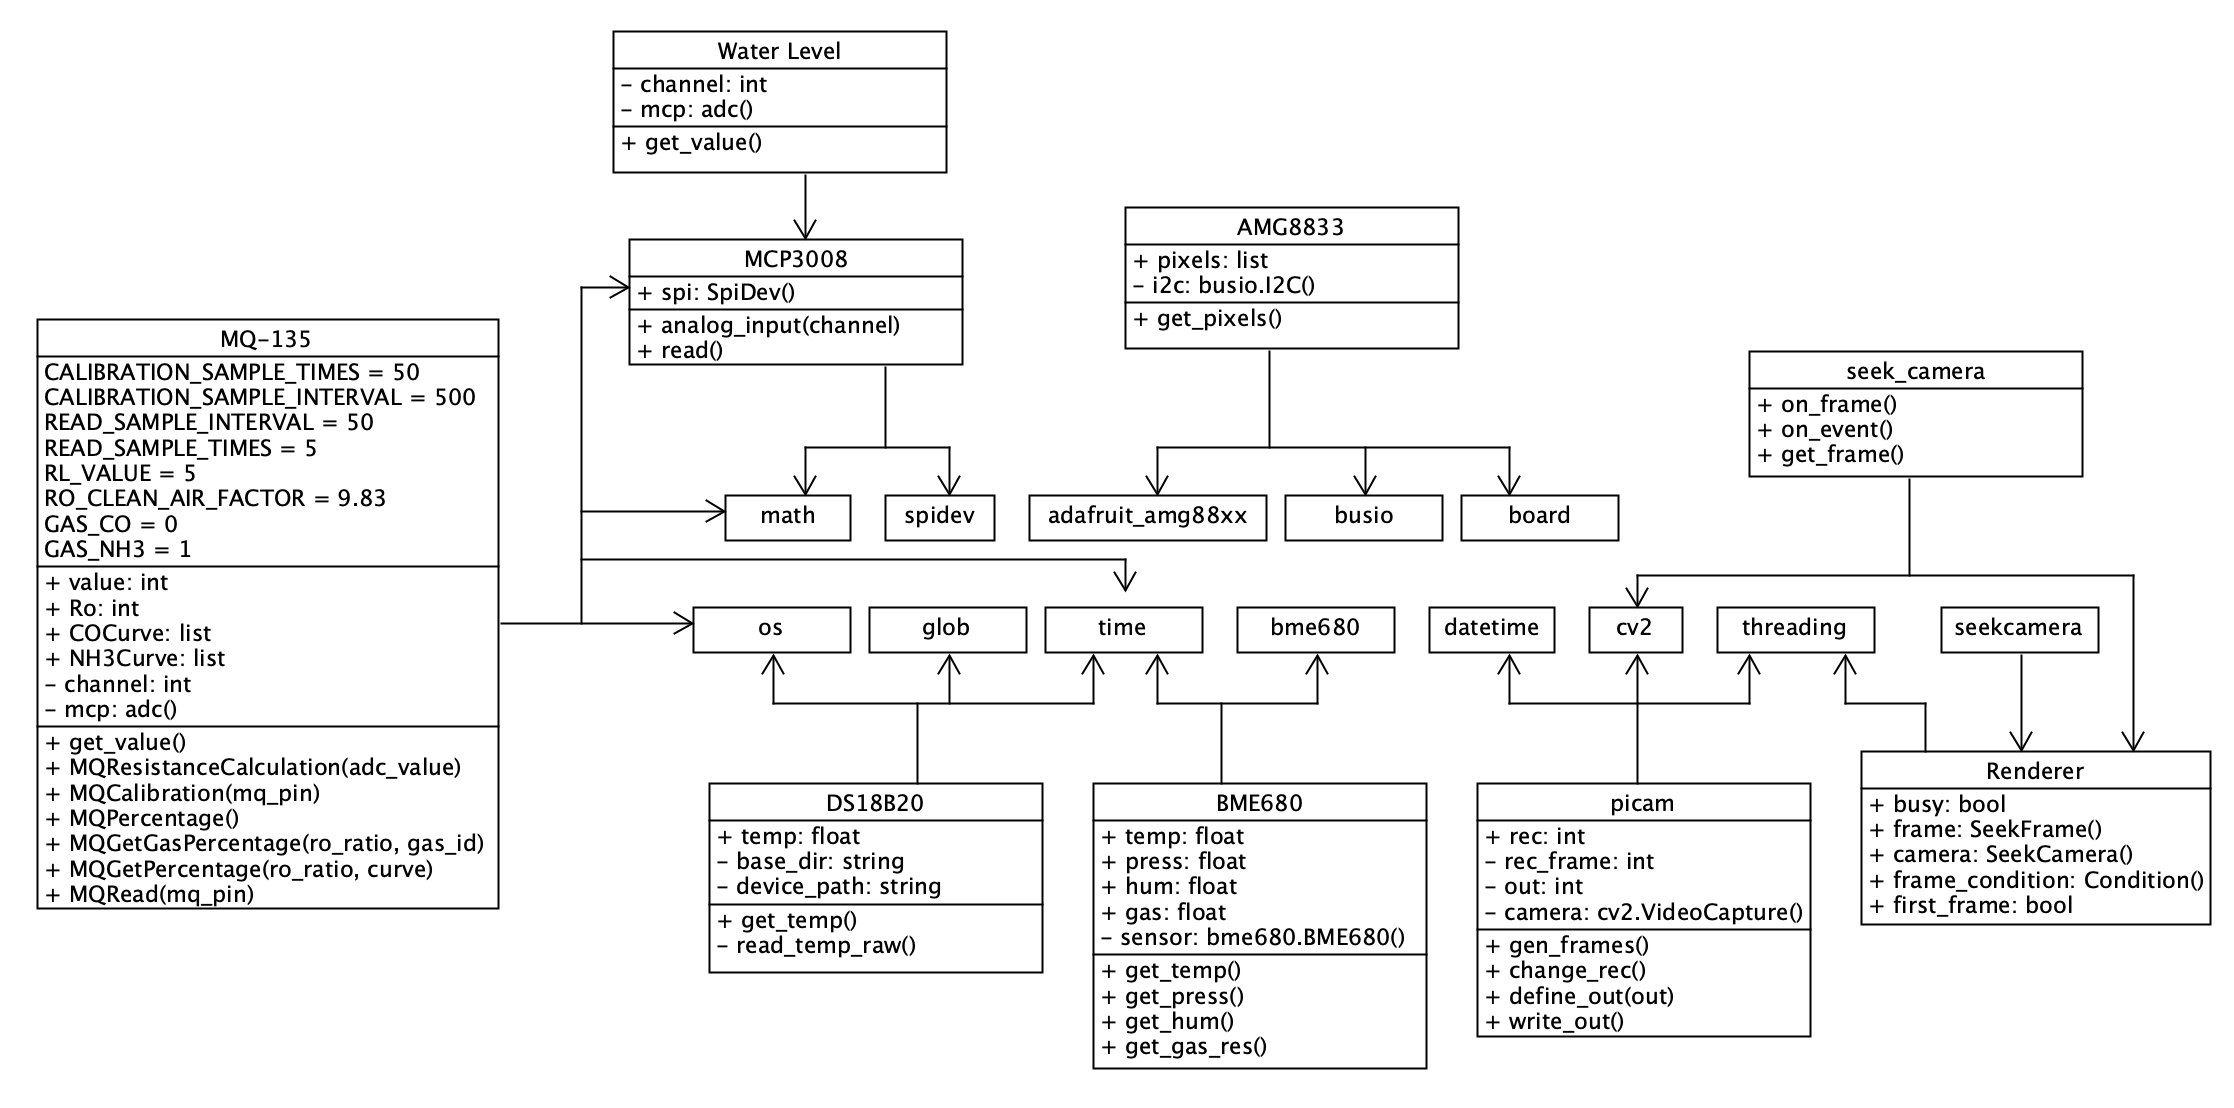
\includegraphics[width=17cm]{figs/umlet}
  \end{center}
  \caption{Diagrama de clases del sistema.}
  \label{fig:umlet}
\end{figure}

En primer lugar, ha sido necesaria la instalación de distintas librerías que dan soporte a los diferentes sensores. Tras la instalación han surgido varios problemas al intentar leer algunos sensores. Uno de los problemas encontrado en dos sensores ---los que funcionaban con conexión I2C--- ha sido que la Raspberry no los detectaba. Se puede encontrar una descripción detallada de los errores que han surgido durante la instalación de las librerías y las respectivas soluciones para hacer funcionar todos los sensores en la wiki\footnote{\url{https://github.com/jmvega/tfg-icebollada/wiki/2.February-progress}} que se ha creado para el proyecto.\\

Durante este proceso, ha habido dos sensores que se han intentado utilizar sin éxito debido a que no tienen compatibilidad con Raspberry: CCS811, que mide la calidad del aire y AM2315, que mide temperatura y humedad. Aun así, esto no ha sido un problema ya que son datos que se han podido obtener con otros sensores.\\

\subsection{Lectura sensorial con Python}
\label{sec:ficheropython}
Dado que el cliente final del sistema puede carecer de nociones avanzadas en informática, es necesario realizar diferentes cambios para ofrecer una comprensión fácil al usuario de los datos obtenidos por los sensores. Se ha utilizado el entorno Node-Red para ofrecer una interfaz amigable al usuario, de forma que este sea capaz de ver la información del estado del sistema representada a través de \textit{widgets}. Este interfaz se ha basado en el diagrama de casos de uso expuesto anteriormente en la Figura \ref{fig:casos}.\\

Para poder mostrar todos los sensores en tiempo real en Node-Red, ha sido necesario disponer de un fichero de Python que cada vez que se ejecute lea una sola vez de todos ellos. No debe leer continuamente ya que es la configuración de Node-Red la que se encarga de ello. En este fichero se procesan todos los sensores menos el AMG8833 (Figura \ref{fig:termicos}-a), la PiCam (Figura \ref{fig:picam_of}) y la cámara térmica (Figura \ref{fig:termicos}-b). Para crear este fichero se ha creado una clase por cada sensor, tal y como se estableció en el diagrama de clases (Figura \ref{fig:umlet}).\\

Este fichero de Python ---indicado como \textit{sensors script} en el diagrama de la Figura \ref{fig:casos}--- utiliza la librería \verb|Threads| para poder leer de manera concurrente todos los sensores, ahorrando tiempo y ganando eficacia. El Código \ref{cod:threads} muestra cómo se crea un hilo ---o \textit{thread}--- por cada sensor.\\
\begin{code}[h]
\begin{lstlisting}[language=Python]
threads = []

#Lista de funciones que devuelven la lectura del sensor respectivo
for func in [x.ammo, x.bme, x.lev, x.water_t]: 
	threads.append(Thread(target=func))
	threads[-1].start()
	
for thread in threads:
	thread.join()
\end{lstlisting}
\caption[Función para crear un Thread por sensor y obtener su lectura.]{Función para crear un Thread por sensor y obtener su lectura.}
\label{cod:threads}
\end{code}

Además, este programa guarda las lecturas en un fichero CSV, por si fuese necesaria la comparación o estudio de datos a lo largo del tiempo. El fichero devuelve una cadena con la lectura de cada sensor (Código \ref{cod:salida}), para poder procesar la salida en Node-Red.\\
\begin{code}[h]
\begin{lstlisting}[language=Python]
Ammonia: 0.91 Temperature: 28.24  Pressure: 1002.1 Humidity: 52.2 Gas: 4005.9 Water level: 2 Waterproof temp: 28.312
\end{lstlisting}
\caption[Ejemplo de salida del fichero Python]{Ejemplo de salida del fichero Python}
\label{cod:salida}
\end{code}

\subsection{Creación de la interfaz de usuario}
\label{sec:IU}
Una vez creado este fichero, se ha procedido a crear la interfaz en Node-Red. Este programa funciona a través de diferentes tipos de nodos, que deben ser combinados para obtener el resultado deseado.\\

En primer lugar, a través del nodo de ejecución, se pueden ejecutar ficheros que están en la máquina local. Este nodo es el que se ha utilizado para integrar en la aplicación el fichero presentado en la Sección \ref{sec:ficheropython}. Para obtener individualmente el valor de cada sensor, se ha utilizado otro nodo ---llamado nodo función--- que permite incluir código directamente en Node-Red. Este nodo se ha utilizado para extraer de la salida del nodo ejecución el valor de interés en cada caso. Este proceso corresponde a las diferentes elipses salientes de \textit{sensors script} del diagrama de casos de uso (Figura \ref{fig:casos}). Con estos dos nodos, algunos sensores han estado listos para mostrar los valores en la interfaz de usuario (IU), por lo que solo ha sido necesario añadir el \textit{widget} más adecuado para cada caso a través del nodo pertinente. Este ha sido el caso de los sensores MQ-135 (Figura \ref{fig:mq_of}), BME680 (Figura \ref{fig:bme_of}) (en el caso de temperatura, presión y humedad) y DS18B20 (Figura \ref{fig:ds_of}).\\

En el caso de los otros sensores, han sido necesarios otros cambios para obtener el resultado adecuado:
\begin{itemize}
	\item El sensor BME680 (Figura \ref{fig:bme_of}) mide la resistencia del gas, pero se ha considerado que no es un parámetro intuitivo y no proporciona conocimiento al usuario. Por ello se ha utilizado otro nodo función que primero realiza la media de 50 lecturas de resistencia de gas y posteriormente establece la calidad del aire en función de la humedad y resistencia del aire comparándolo con la media calculada.
	
	\item Durante diferentes pruebas, se ha detectado que el sensor que mide el nivel de agua (Figura \ref{fig:nivel_of}) no es preciso a la hora de detectar la cantidad de agua presente, solamente es preciso detectando la presencia de esta. Por tanto, se ha optado por dividir en 4 rangos el nivel de agua (Figura \ref{fig:agua}), de tal manera que el usuario tenga una idea sobre la cantidad de agua presente. Aún así, el sensor no es suficientemente preciso durante la realización de diferentes pruebas y esta opción tampoco ha sido válida. Como ajuste que dota de más precisión a este sensor, se ha incorporado un botón en la IU para poder calibrar el sensor cuando el recipiente esté lleno de agua. Todo el desarrollo y las pruebas que se han llevado a cabo con este sensor pueden ser encontradas en la wiki\footnote{\url{https://github.com/jmvega/tfg-icebollada/wiki/3.March-progress}} del proyecto.
	
	\item El sensor AMG8833 (Figura \ref{fig:termicos}-a) devuelve en su lectura una matriz de 8x8 valores. Estos valores han sido convertidos a imagen ya que este sensor es una cámara térmica. Para este proceso ha sido necesario enlazar una serie de nodos hasta poder obtener la imagen más nítida (Figura \ref{fig:temps}), ya que la imagen obtenida originalmente ha sido una imagen de 8x8 píxeles que no alcanzaba a diferenciar objetos. De nuevo, tanto este progreso como las diferentes soluciones obtenidas se pueden encontrar en la wiki. 
\end{itemize}
\begin{figure}[h!]
  \begin{center}
    \subfigure[]{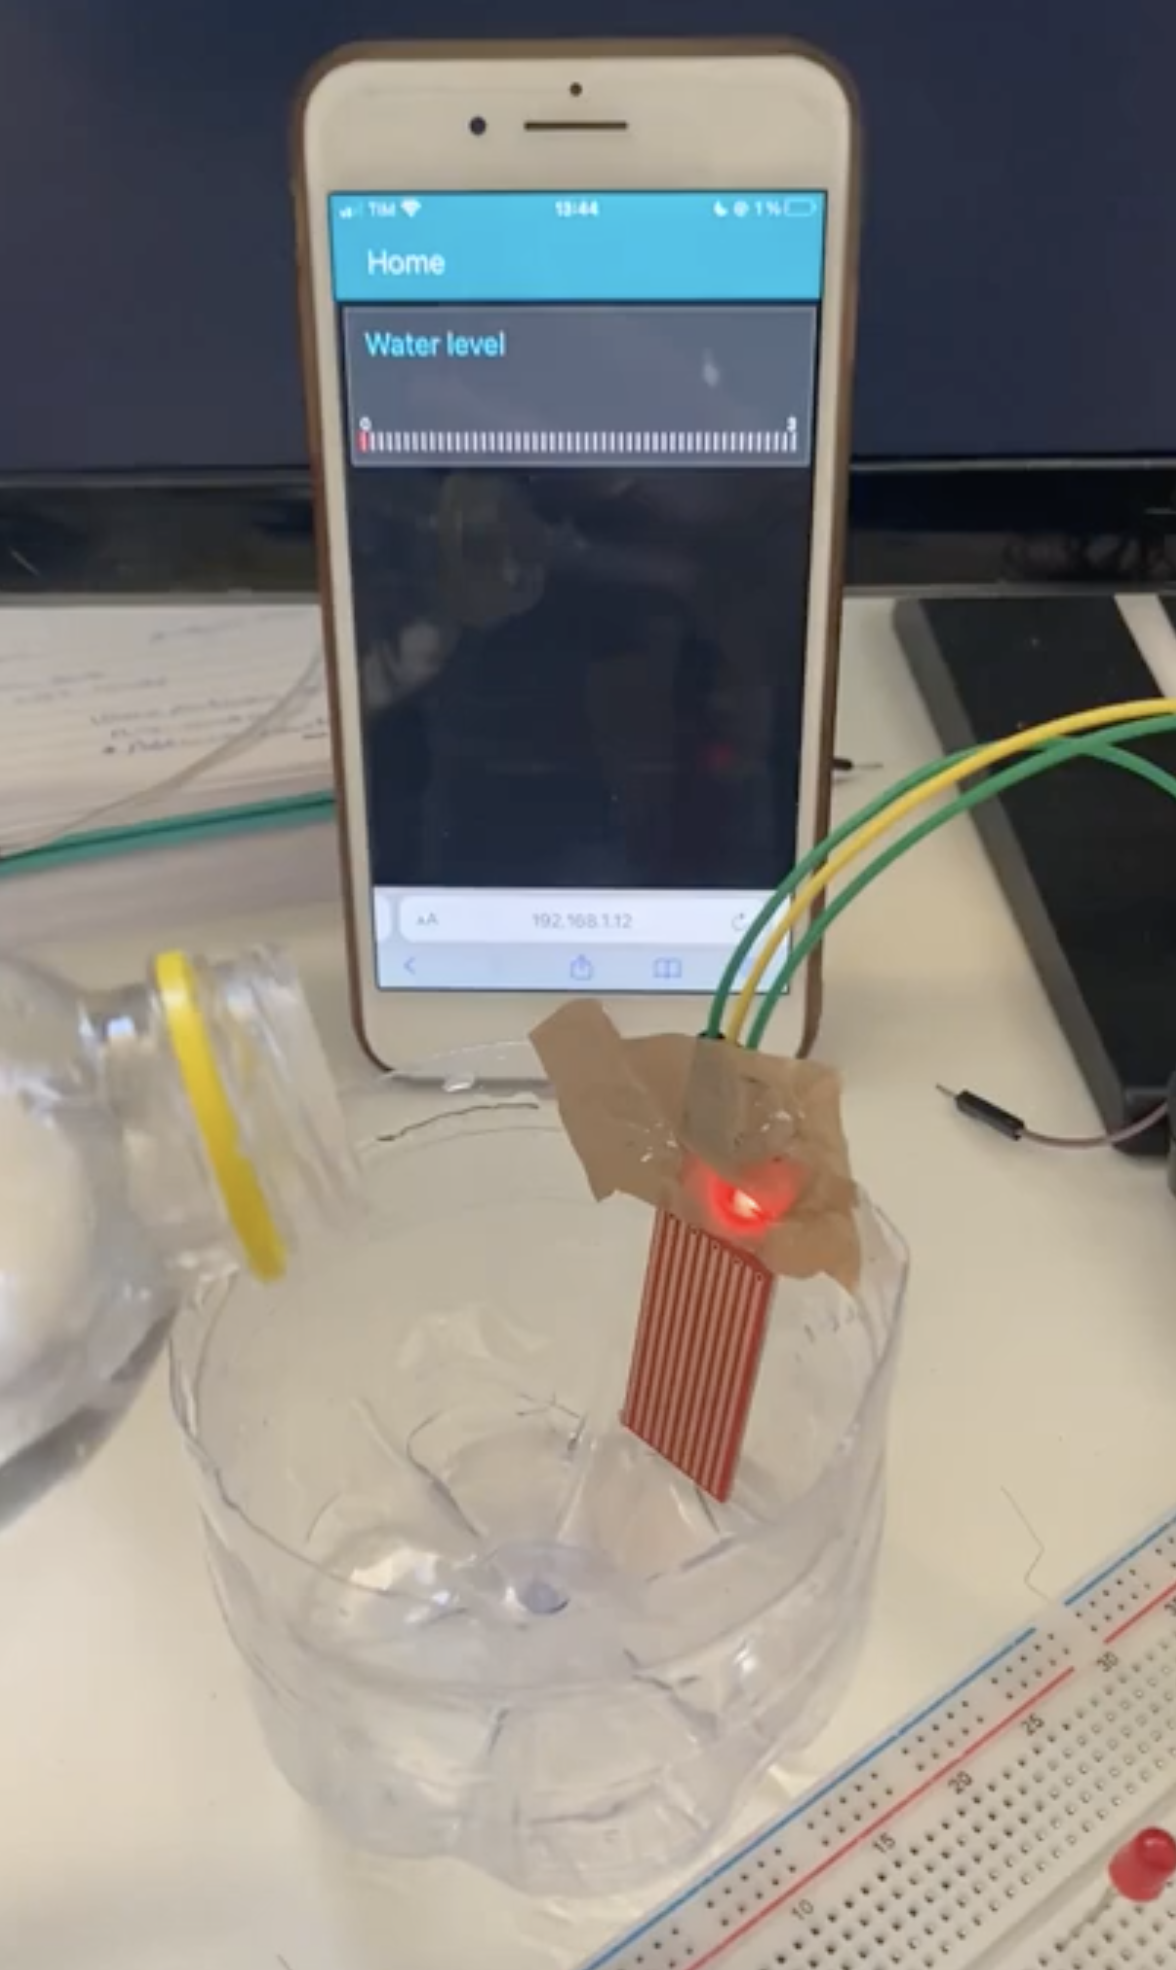
\includegraphics[width=3.4cm]{figs/agua1}}\hspace{1mm}
    \subfigure[]{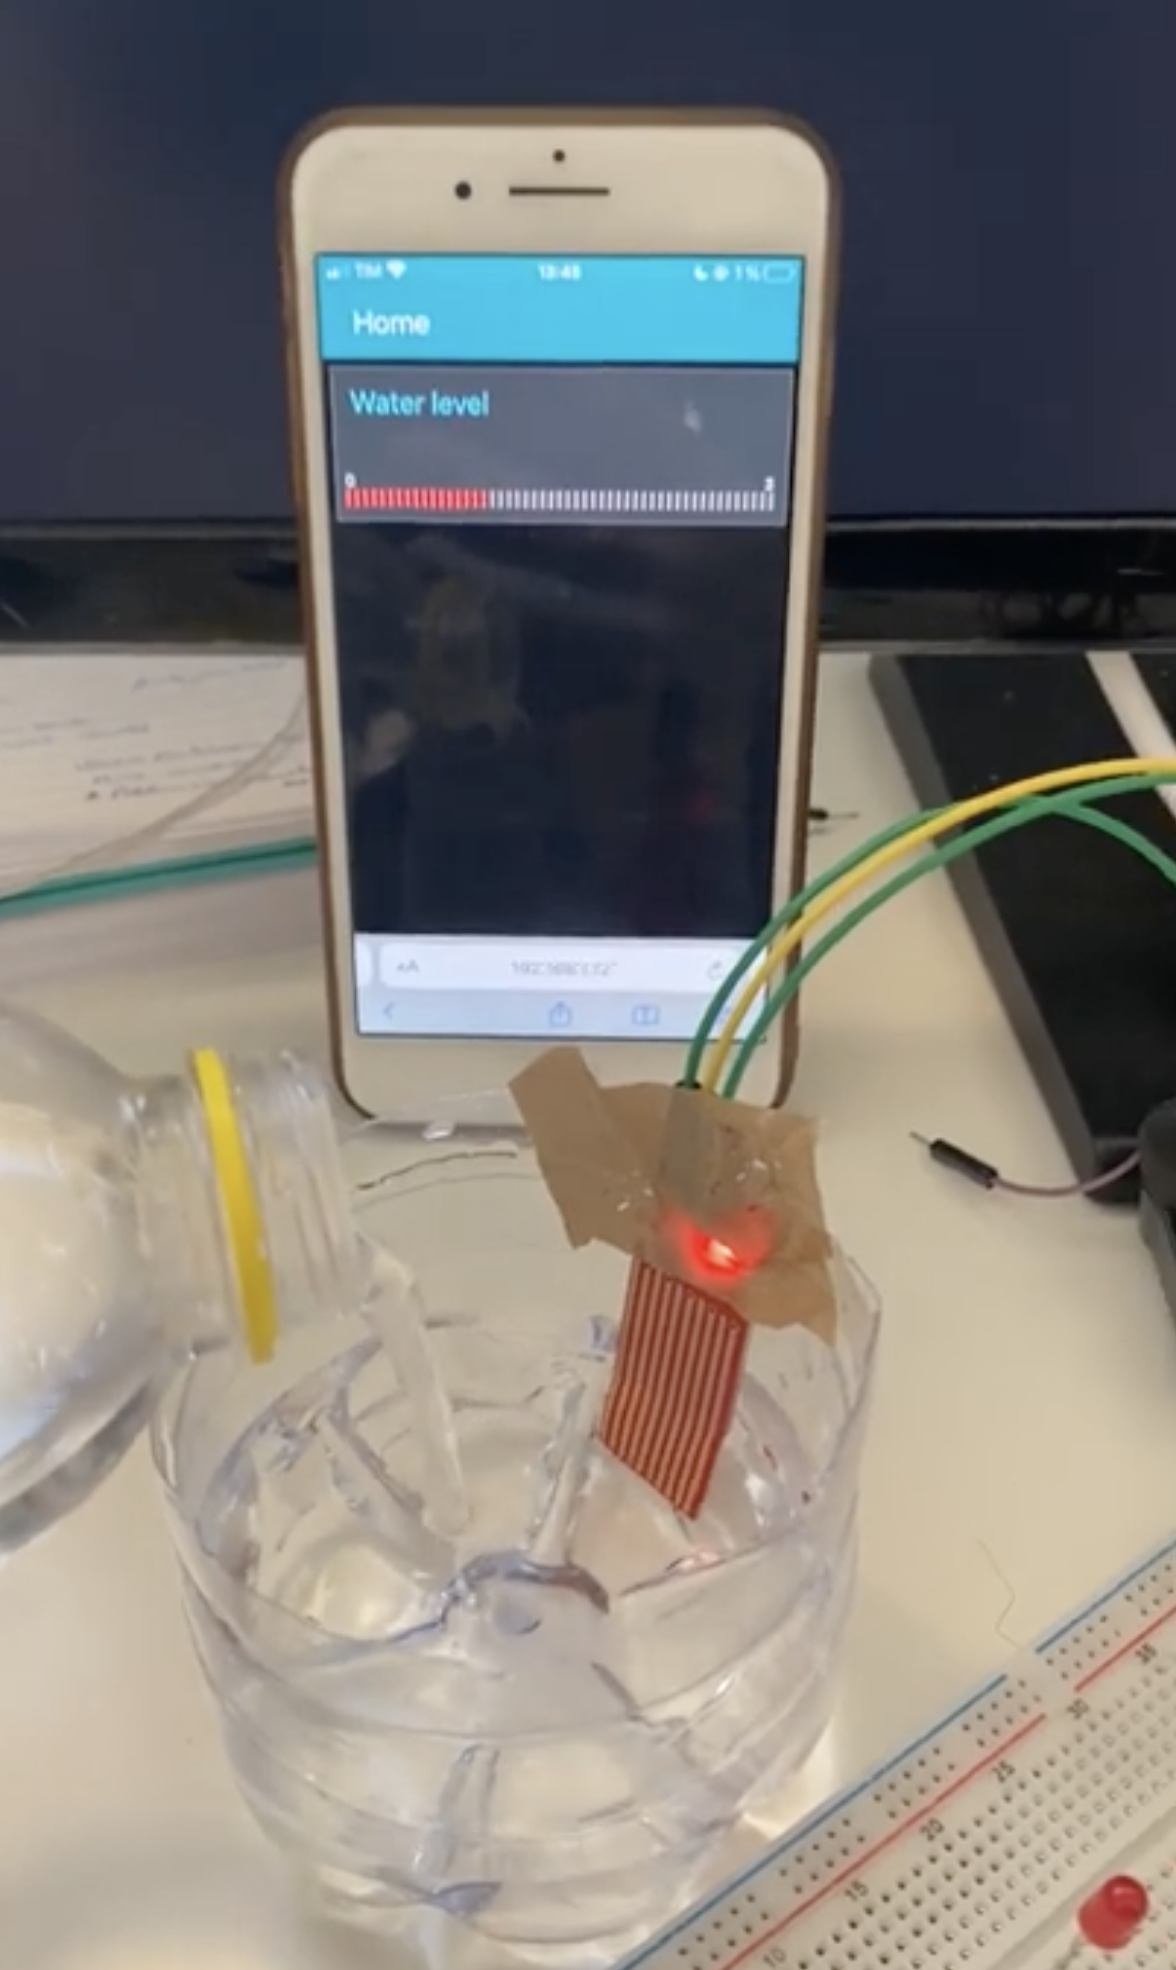
\includegraphics[width=3.4cm]{figs/agua2}}\hspace{1mm}
    \subfigure[]{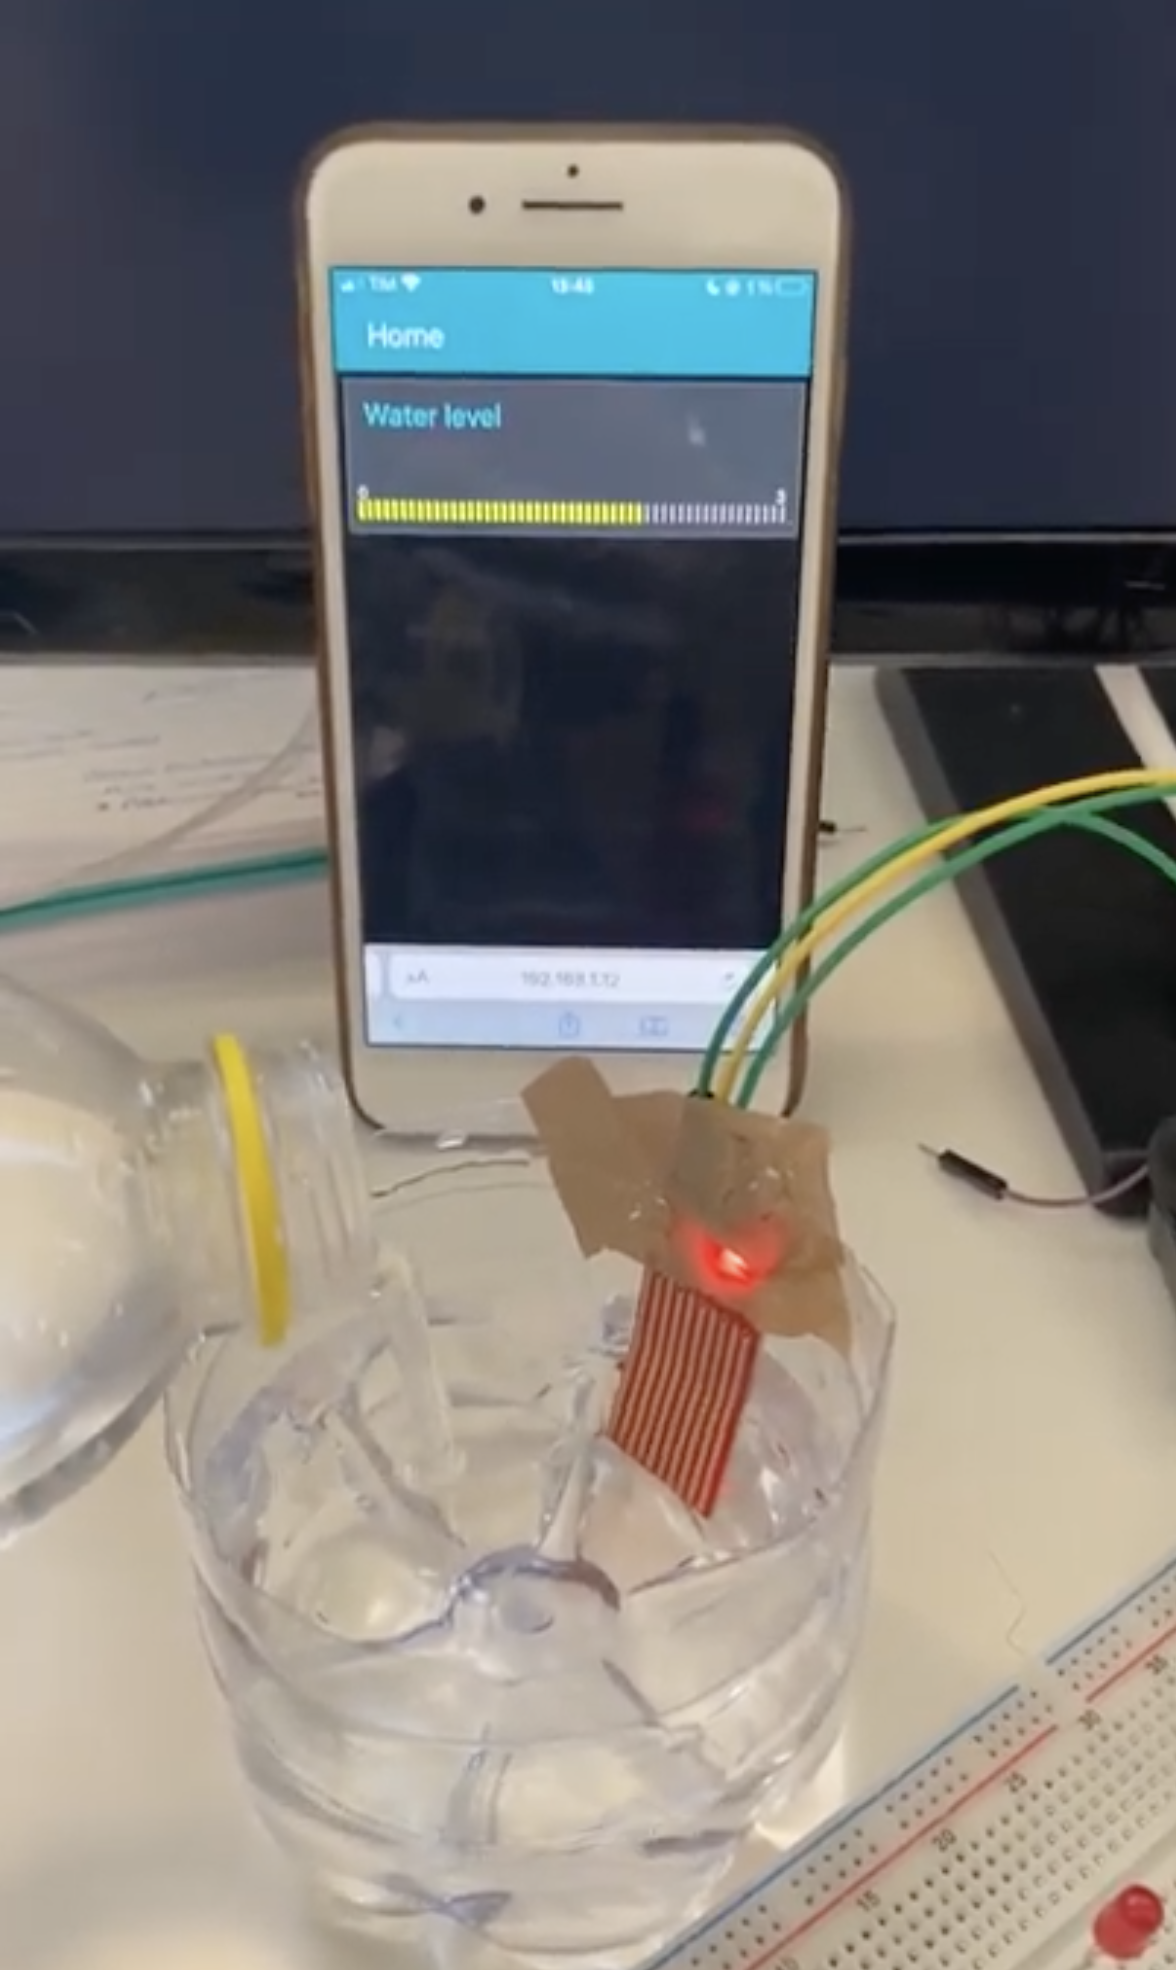
\includegraphics[width=3.4cm]{figs/agua3}}\hspace{1mm}
    \subfigure[]{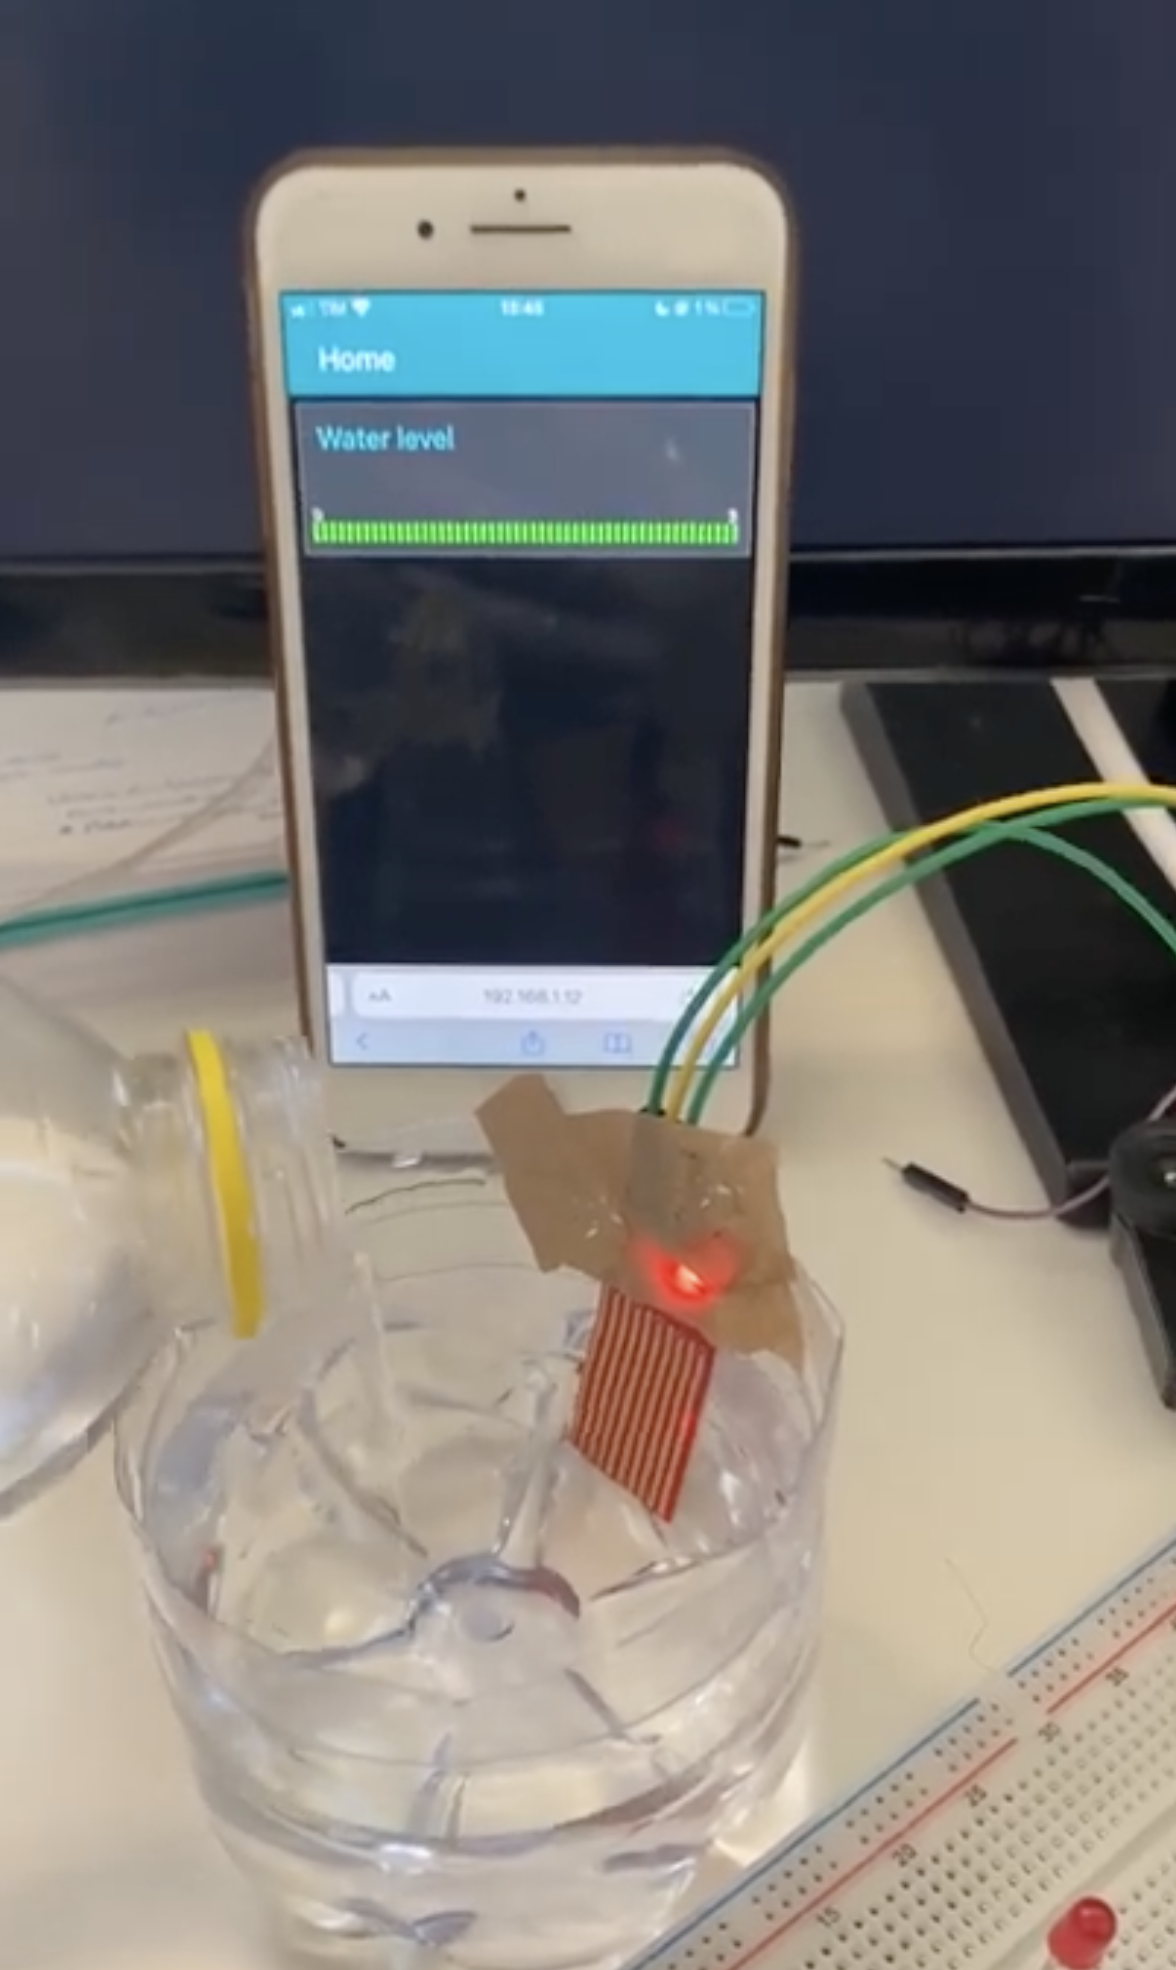
\includegraphics[width=3.4cm]{figs/agua4}}
  \end{center}
\caption{Proceso de indicación del nivel de agua.} \label{fig:agua}
\end{figure}

 \begin{figure} [h!]
  \begin{center}
    \includegraphics[width=8cm]{figs/temps}
  \end{center}
  \caption{Imagen generada después de la conversión de los datos numéricos.}
  \label{fig:temps}
\end{figure}

Con estos ajustes realizados, se ha obtenido parte de la IU. Para hacerla más completa se ha incorporado un interruptor de forma que el usuario puede decidir si apagarla o bien mantenerla encendida, así como un nodo que regula la repetitividad del sistema cada 3 segundos. La interfaz formada por los sensores comentados previamente se puede ver en la Figura \ref{fig:ui_nocams}.
\begin{figure} [h!]
  \begin{center}
    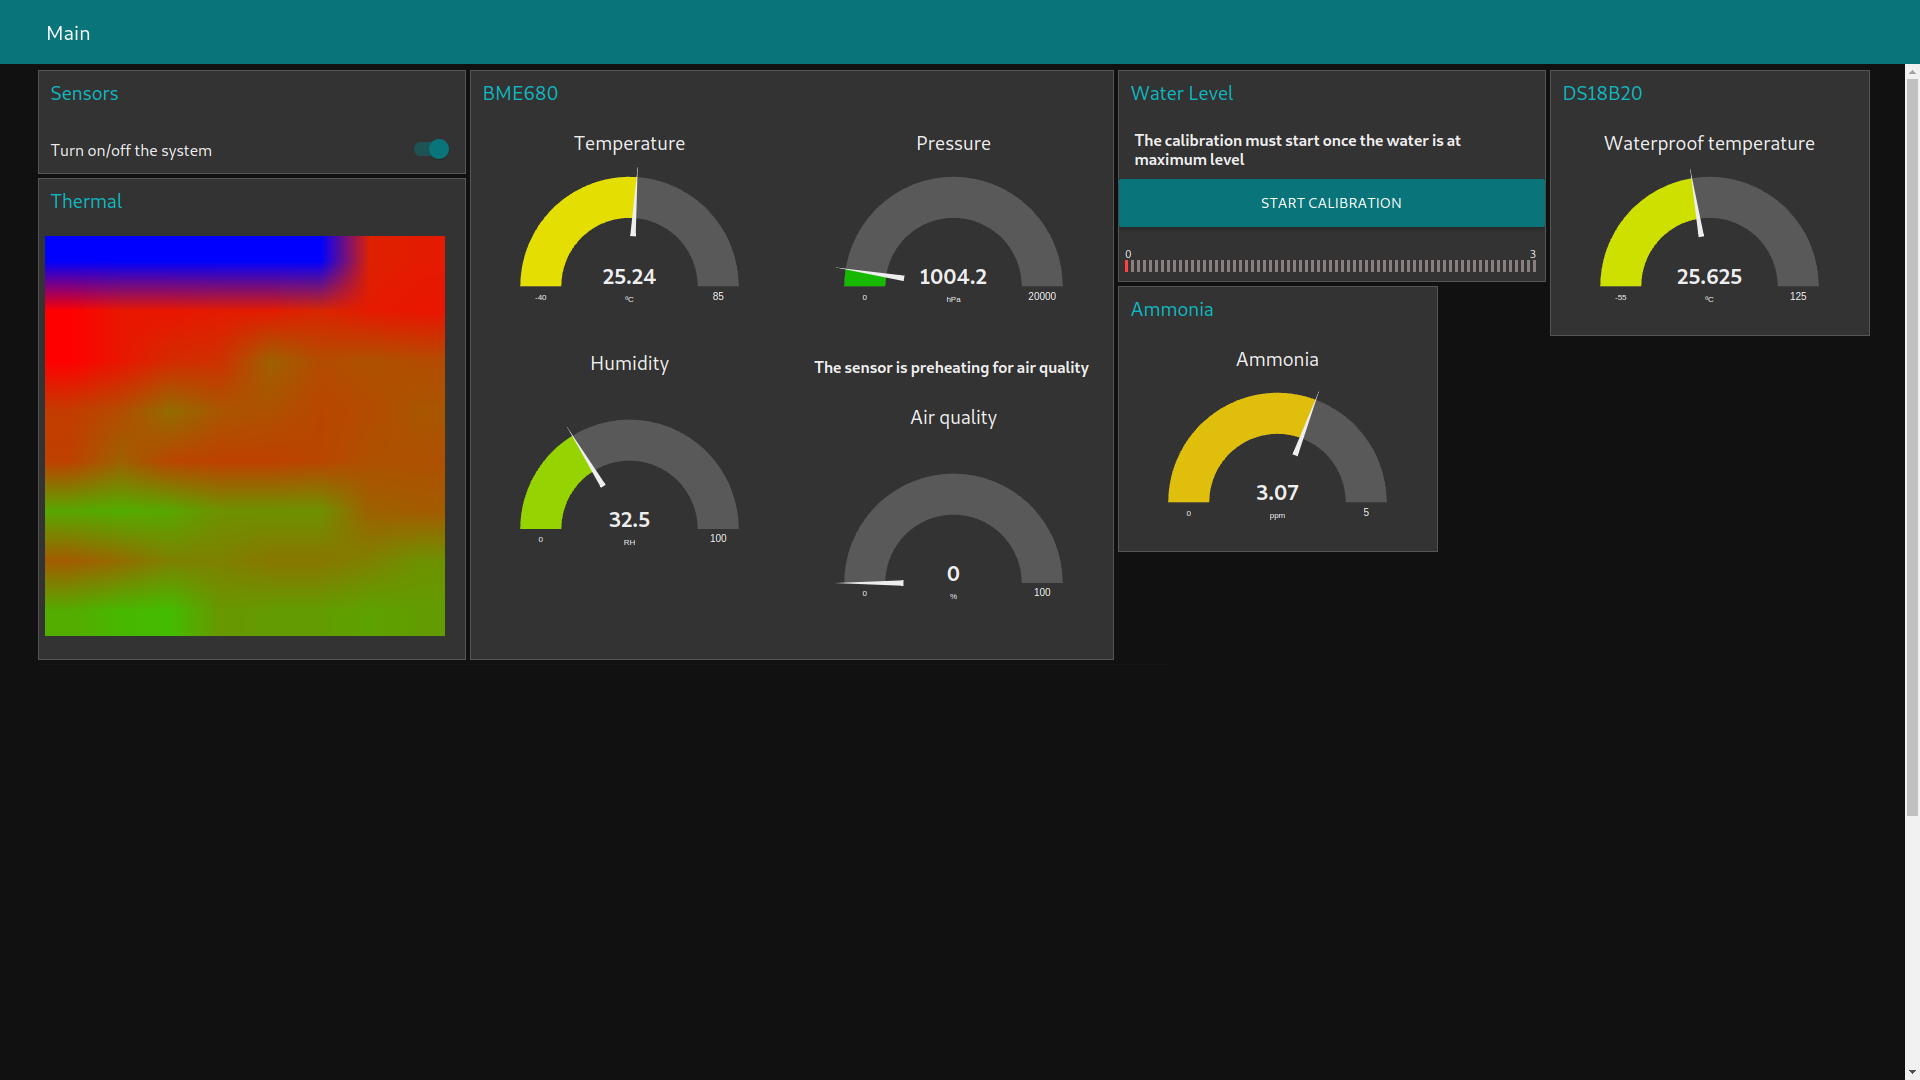
\includegraphics[width=16cm]{figs/ui_nocams}
  \end{center}
  \caption{IU sin los canvas correspondientes a la utilización de las cámaras.}
  \label{fig:ui_nocams}
\end{figure}

\subsection{Integración de las cámaras en la IU}
La creación de la interfaz, descrita en la Sección \ref{sec:IU} no es completa, ya que faltan dos de los sensores que se utilizan en este trabajo: las cámaras. Para poder visualizar las cámaras desde Node-Red debe ser a través del nodo \textit{template} (plantilla), que permite visualizar una dirección web. Por tanto, ha sido necesario crear un servidor que permita visualizar las imágenes de las dos cámaras y, con ello, poder incluirlo en la IU. Para crear este servidor se ha utilizado Flask.\\

Se ha decidido crear un servidor por cada cámara. De esta manera se puede acceder solamente a una visualización o bien a las dos, según el interés del usuario. Para el funcionamiento de la cámara térmica Seek Thermal (Figura \ref{fig:termicos}-b) se ha utilizado la librería que tiene Seek, que permite su visualización a través de OpenCV. Para el funcionamiento de la PiCam (Figura \ref{fig:picam_of}) se ha utilizado OpenCV, tanto para su visualización como para la incrustación de la fecha y la hora en las imágenes (Figura \ref{fig:fechayhora}). El Código \ref{cod:fechayhora} muestra cómo se consigue.\\
\begin{figure} [h!]
  \begin{center}
    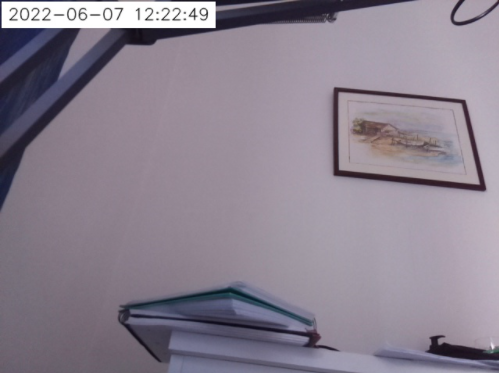
\includegraphics[width=8cm]{figs/fechayhora}
  \end{center}
  \caption{Incorporación de la fecha y hora en la visualización de la PiCam.}
  \label{fig:fechayhora}
\end{figure}

\begin{code}[h]
\begin{lstlisting}[language=Python]
ret, frame = self.__camera.read()
frame = cv2.rectangle(frame, (2,2), (275,35), (255,255,255), -1)
frame = cv2.putText(frame, str(datetime.datetime.now().replace(microsecond=0)), (10,25), cv2.FONT_HERSEY_SIMPLEX, 0.7, (0,0,0), 1, cv2.LINE_AA))
\end{lstlisting}
\caption[Código para incorporar la fecha en la esquina superior izquierda.]{Código para incorporar la fecha en la esquina superior izquierda.}
\label{cod:fechayhora}
\end{code}

Una vez obtenidas las imágenes de las cámaras desde la Raspberry, se ha incorporado al código el uso de Flask para poder crear el servidor. Es necesario disponer de dos elementos: el código para mostrar la imagen de la cámara, y una carpeta donde están las plantillas. Estas plantillas son ficheros escritos en lenguaje HTML que muestran en el servidor la página que interesa en cada momento. La estructura que sigue un programa con Flask es la representada en el Código \ref{cod:flask}.\\
\begin{code}[h]
\begin{lstlisting}[language=Python]
from flask import *
app = Flask(__name__)

@app.route('/')
def home():
   return render_template('index.html')

if __name__ == '__main__':
   app.run(host='0.0.0.0', port=8000, debug=True)
\end{lstlisting}
\caption[Creación de un servidor web en el puerto 8000.]{Creación de un servidor web en el puerto 8000.}
\label{cod:flask}
\end{code}

Después de incorporar el código del funcionamiento de cada cámara en los respectivos servidores, se ha añadido un botón para iniciar o parar la grabación del vídeo en la cámara normal. Para diferenciar cuándo se está grabando de cuándo no, se ha añadido un mensaje en pantalla indicando que se está grabando. El vídeo se guarda en la Raspberry de forma local y en formato .avi. En la Figura \ref{fig:proceso} se puede ver el proceso de registro en el servidor para acceder a la visualización de la PiCamera.\\
\begin{figure}[h!]
  \begin{center}
    \subfigure[Pantalla inicial del servidor]{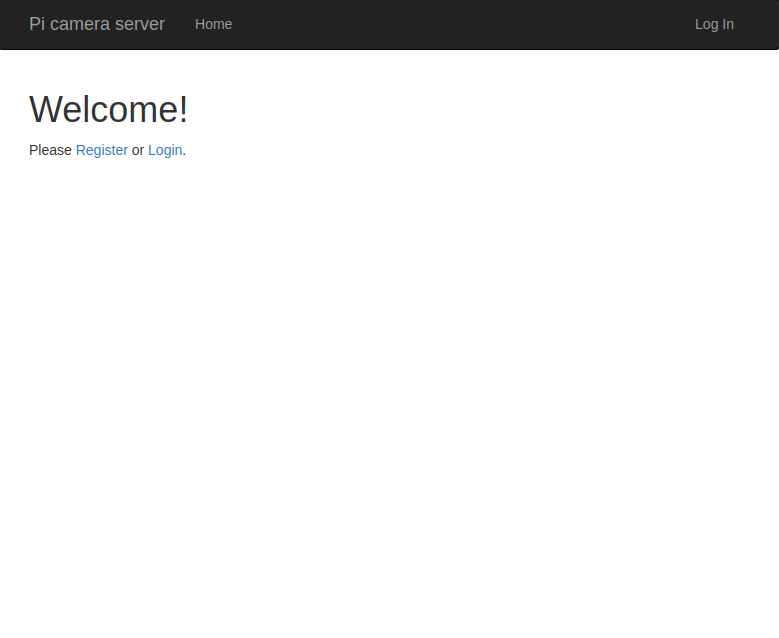
\includegraphics[width=7cm]{figs/server1}}\hspace{1mm}
    \subfigure[Pantalla de registro]{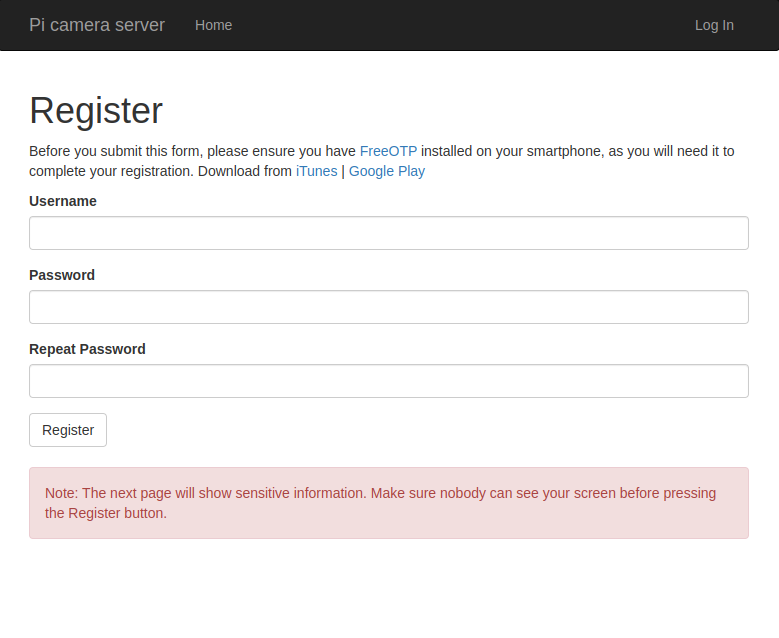
\includegraphics[width=7cm]{figs/server2}}\hspace{2mm}
    \subfigure[Código de doble autenticación]{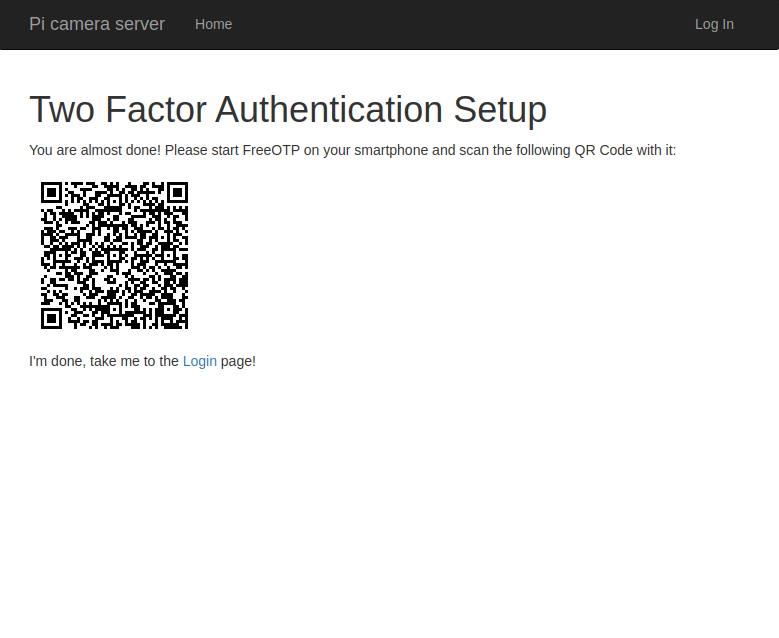
\includegraphics[width=7cm]{figs/server3}}\hspace{1mm}
    \subfigure[Escaneo de código]{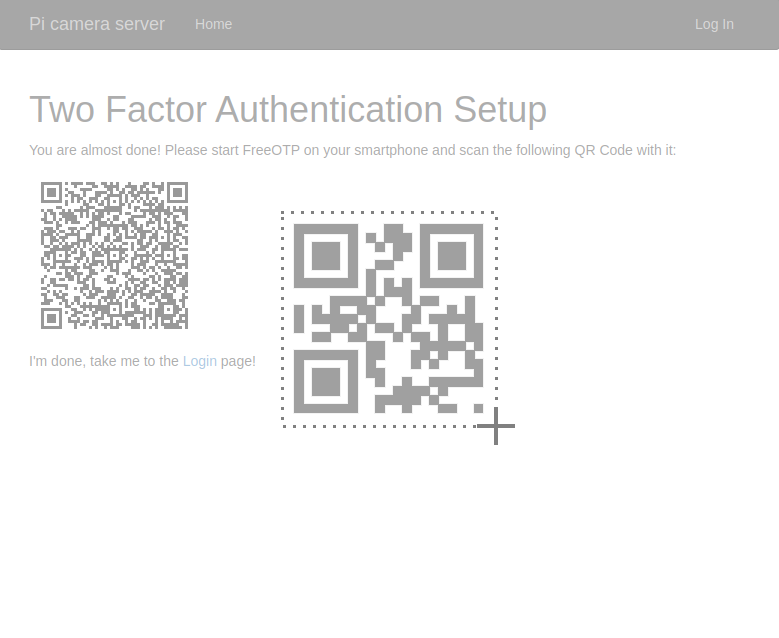
\includegraphics[width=7cm]{figs/server4}}
    \subfigure[Pantalla de login]{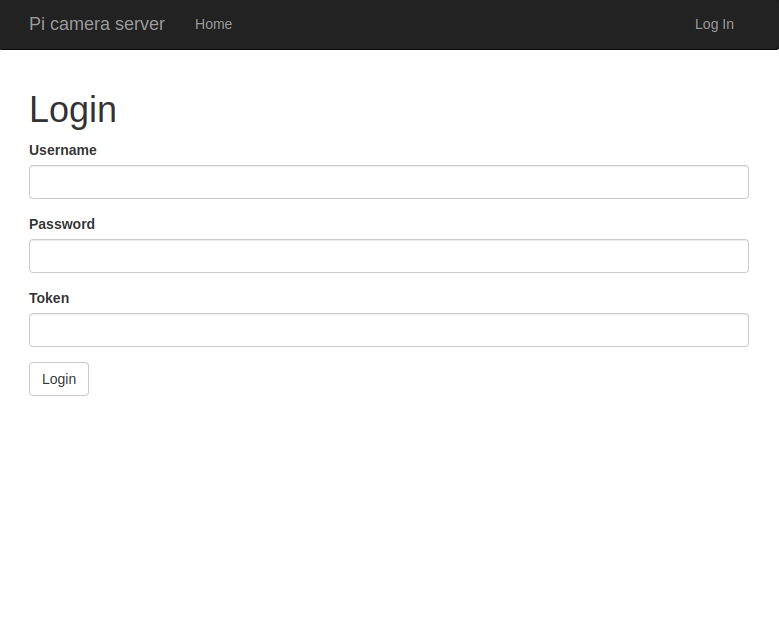
\includegraphics[width=7cm]{figs/server6}}\hspace{2mm}
    \subfigure[Visualización de la cámara]{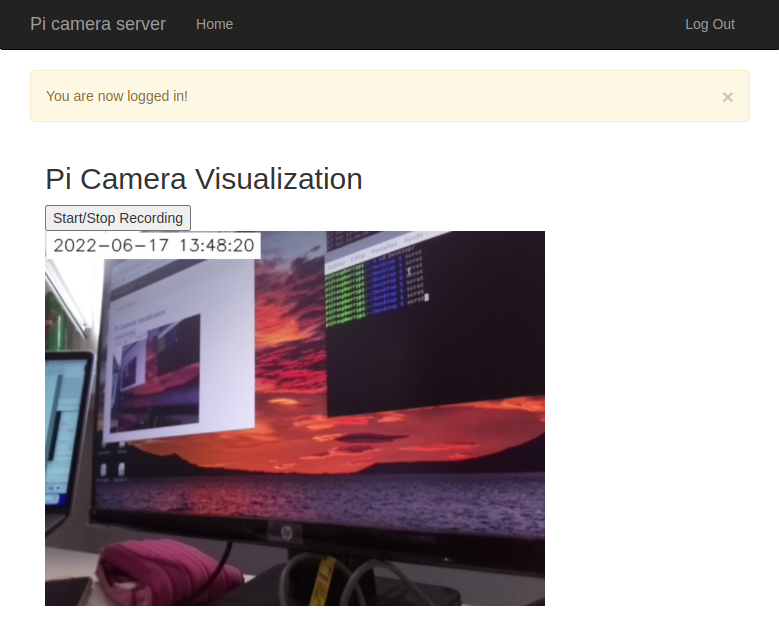
\includegraphics[width=7cm]{figs/server7}}
  \end{center}
\caption{Proceso de registro en el servidor de Flask de la PiCam.} \label{fig:proceso}
\end{figure}

Una vez se ha obtenido la visualización de las cámaras en la IU junto al resto de sensores, la interfaz está completada siguiendo la estructura presentada en el diagrama de casos de uso (Figura \ref{fig:casos}).


\subsection{Seguridad}
Debido a que se está trabajando en un servidor web, es importante dotar de cierta seguridad a este para que sólo las personas autorizadas puedan acceder a las imágenes. Para ello, se ha implementado el factor de doble autenticación (del inglés Two Factor Authentication, 2FA). 2FA es el proceso de autenticación donde se añade un segundo paso en el proceso de identificación frente a un servicio (por ejemplo, mediante el envío de un SMS de confirmación). En este caso, además de que un usuario introduzca su contraseña, es necesario un código que se genera cada 30 segundos y caduca pasado ese tiempo. La generación de este código se hace a través de Google Authenticator\footnote{\url{https://chrome.google.com/webstore/detail/authenticator/bhghoamapcdpbohphigoooaddinpkbai?hl=es}}. Esta extensión de Google genera los códigos (de 30 segundos de vida) a partir del escaneo de un código QR (Figura \ref{fig:proceso}-d).\\

Para que estos servidores funcionen con 2FA, ha sido necesario incorporar otras librerías, así como otros módulos de Flask: \textit{Flask\_login}, \textit{Flask\_bootstrap}, \textit{Flask\_sqlalchemy} y \textit{Flask\_wtf}. Durante el desarrollo del servidor con 2FA han surgido determinados problemas, que pueden encontrarse junto a la solución en la wiki del proyecto\footnote{\url{https://github.com/jmvega/tfg-icebollada/wiki/5.May-progress}}.\\

Una vez los servidores web han funcionado, se han integrado en Node-Red a través del nodo \textit{template}. Un servidor está en el puerto 5000 y, el otro, en el 8000, para que así puedan estar ambas cámaras disponibles a la vez. Una vez añadidos, la interfaz de usuario (Figura \ref{fig:UIcompleta}) queda completa.\\
\begin{figure} [h!]
  \begin{center}
    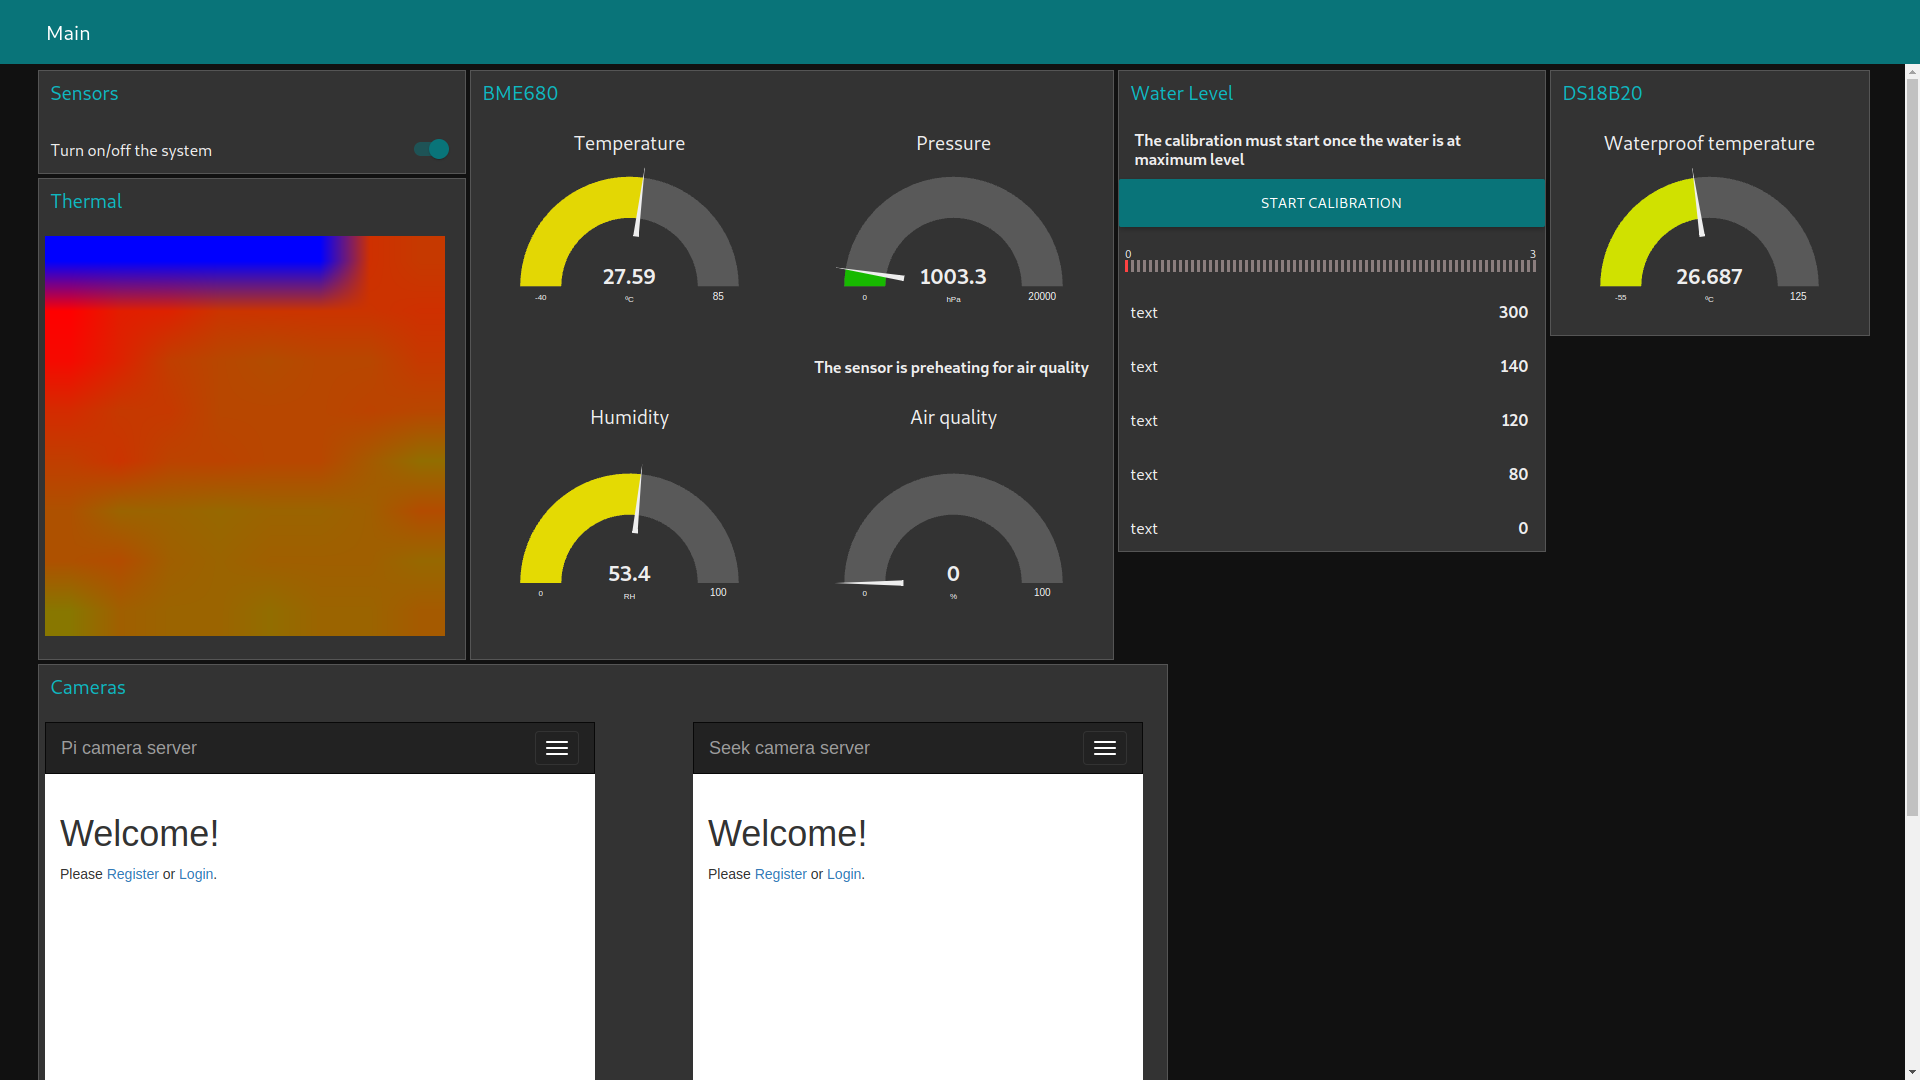
\includegraphics[width=16cm]{figs/UIcompleta}
  \end{center}
  \caption{Visualización de la interfaz de usuario.}
  \label{fig:UIcompleta}
\end{figure}

También se ha incorporado seguridad en Node-Red, ya que este funciona sobre una dirección a la que puede acceder cualquier usuario de la red sobre el puerto 1880. Por tanto, es imprescindible que sean solo los usuarios autorizados los que puedan acceder a esta plataforma, sobre todo en la parte del flujo de nodos. Así, se ha optado por dividir este acceso en dos partes. Una de ellas, la parte de administrador (Figura \ref{fig:adminlogin}), donde se encuentra el flujo de nodos y se crea toda la interfaz de usuario; únicamente un administrador debe poder acceder a esta parte, ya que es importante que una persona que no tiene conocimientos acerca de su funcionamiento no pueda realizar modificaciones. La otra parte corresponde a la interfaz de usuario (Figura \ref{fig:userlogin}); solo un usuario registrado conocedor de la contraseña puede acceder al sistema. Tanto las contraseñas de Node-Red como las de los servidores se guardan encriptadas bajo algoritmos de funciones hash en SHA256.\\ 
\begin{figure}[h!]
  \begin{center}
    \subfigure[]{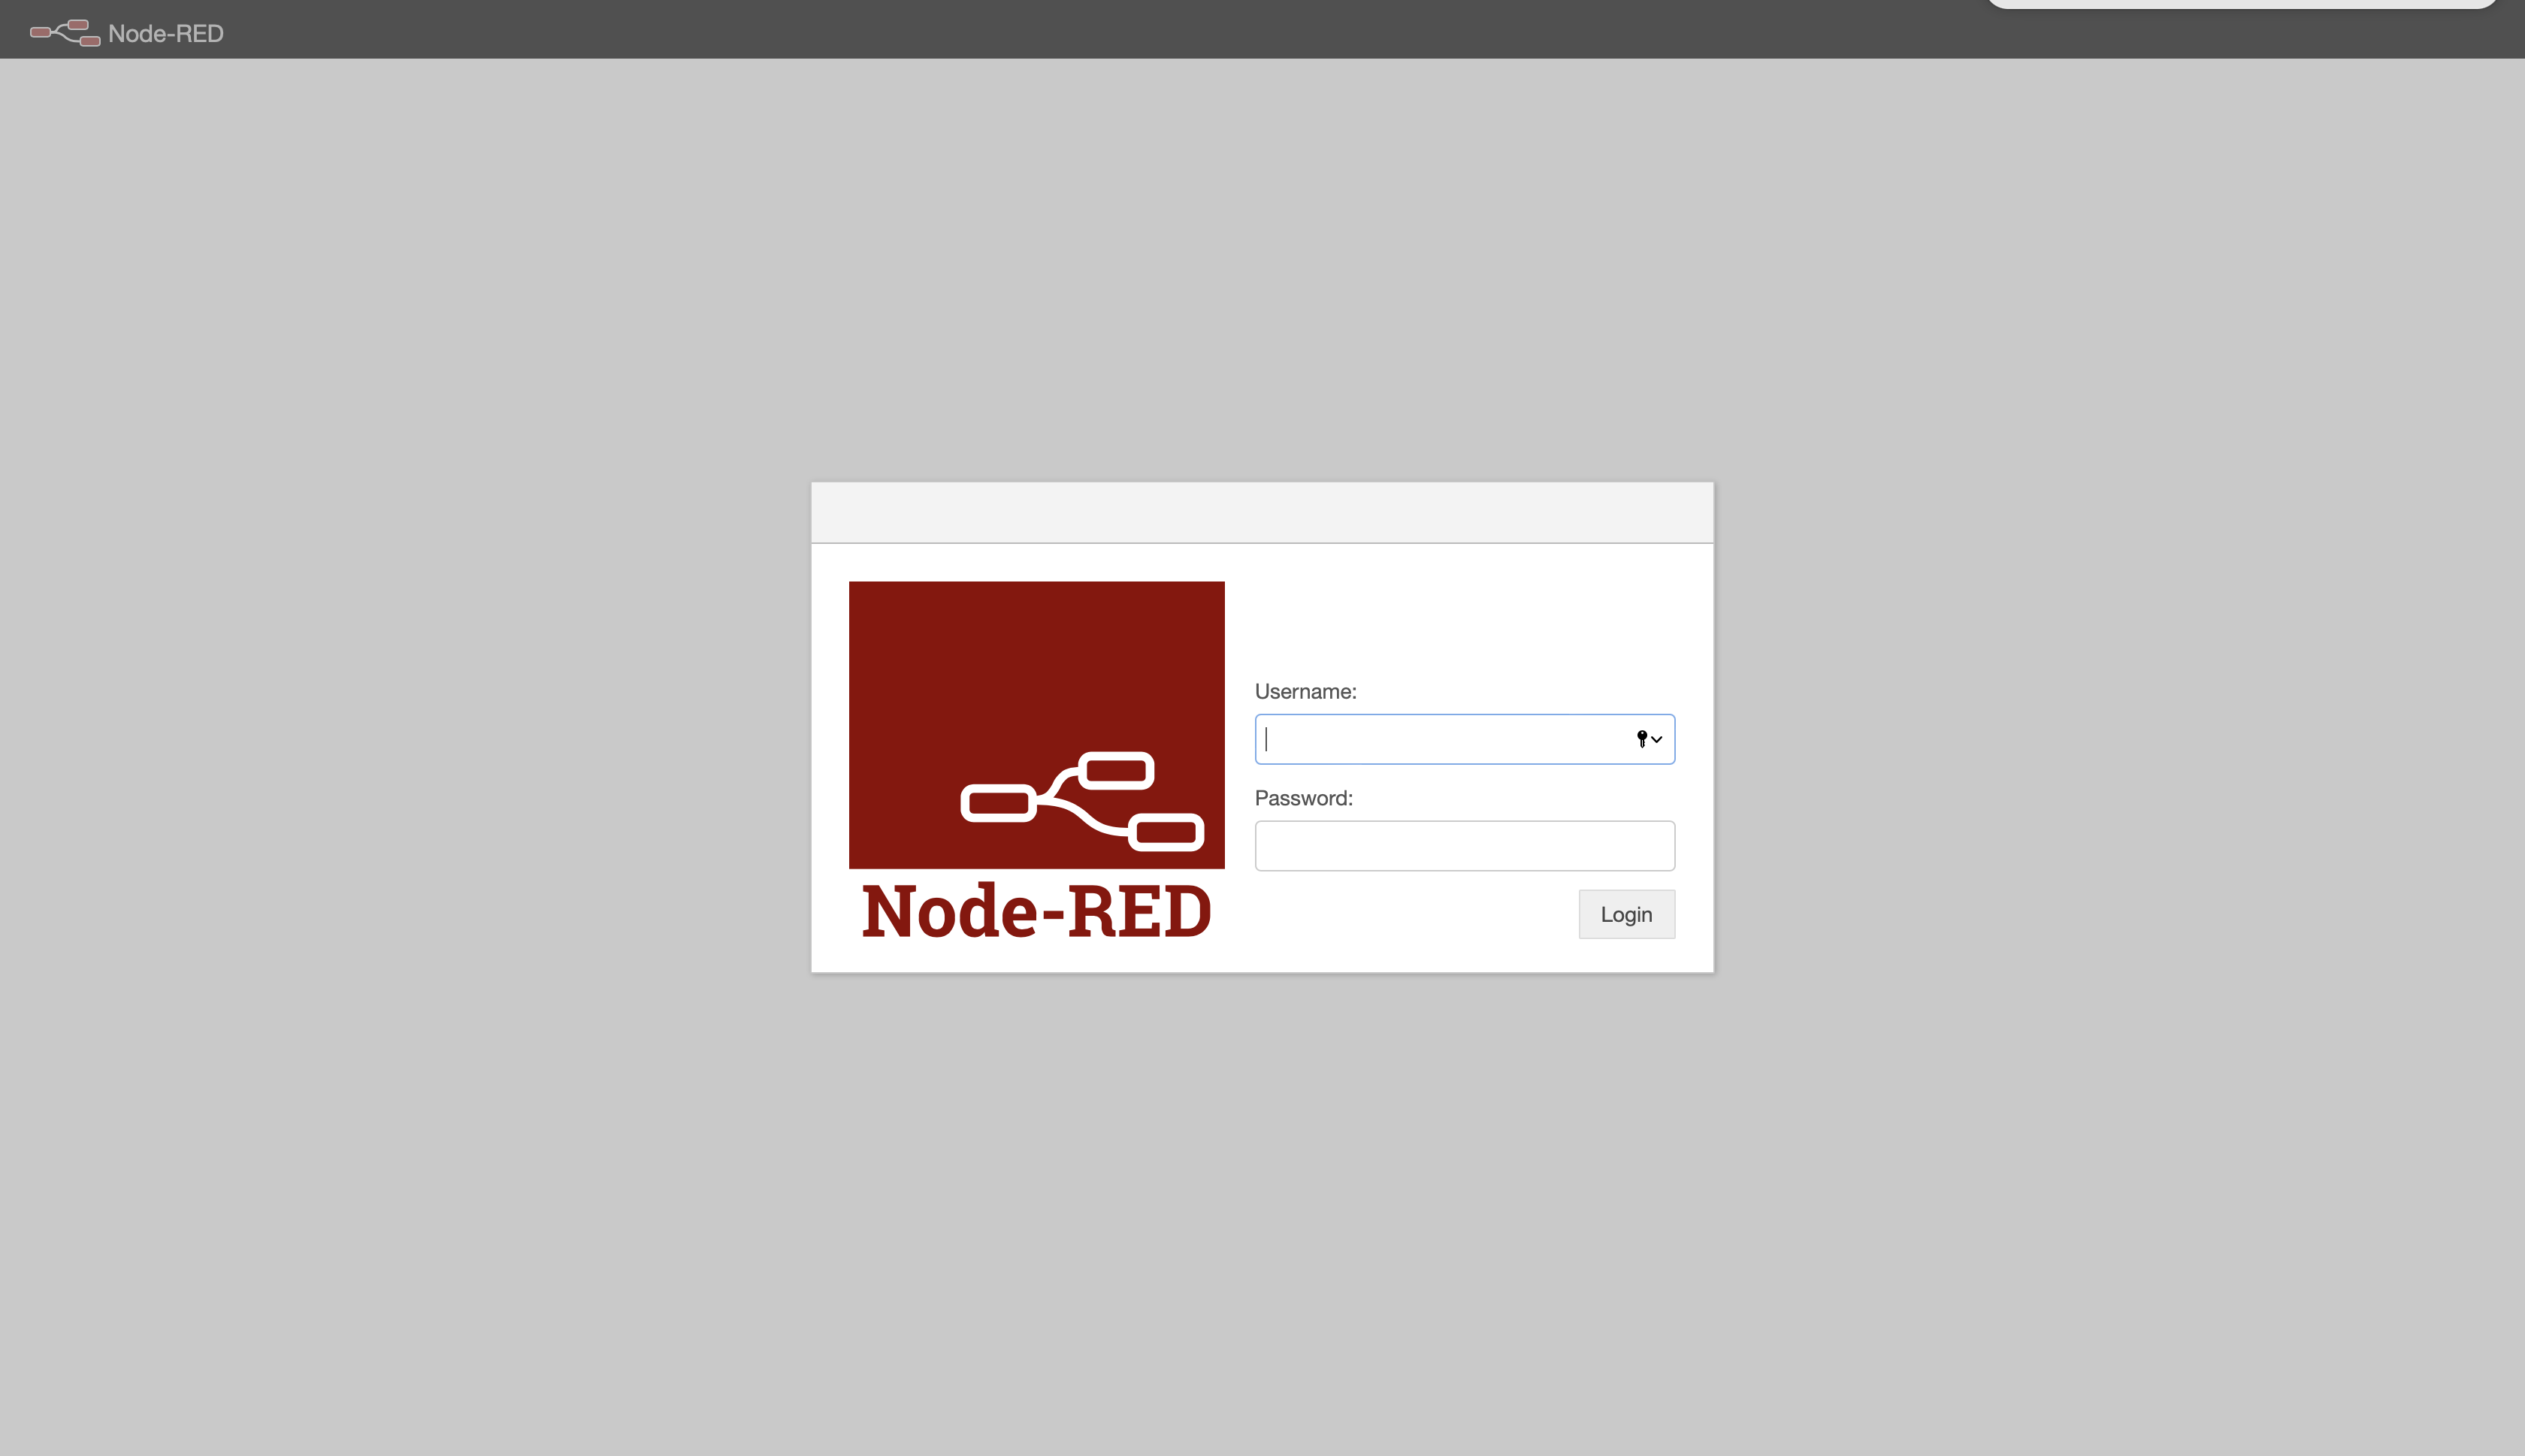
\includegraphics[width=12cm]{figs/nodered-1}}\hspace{2mm}
    \subfigure[]{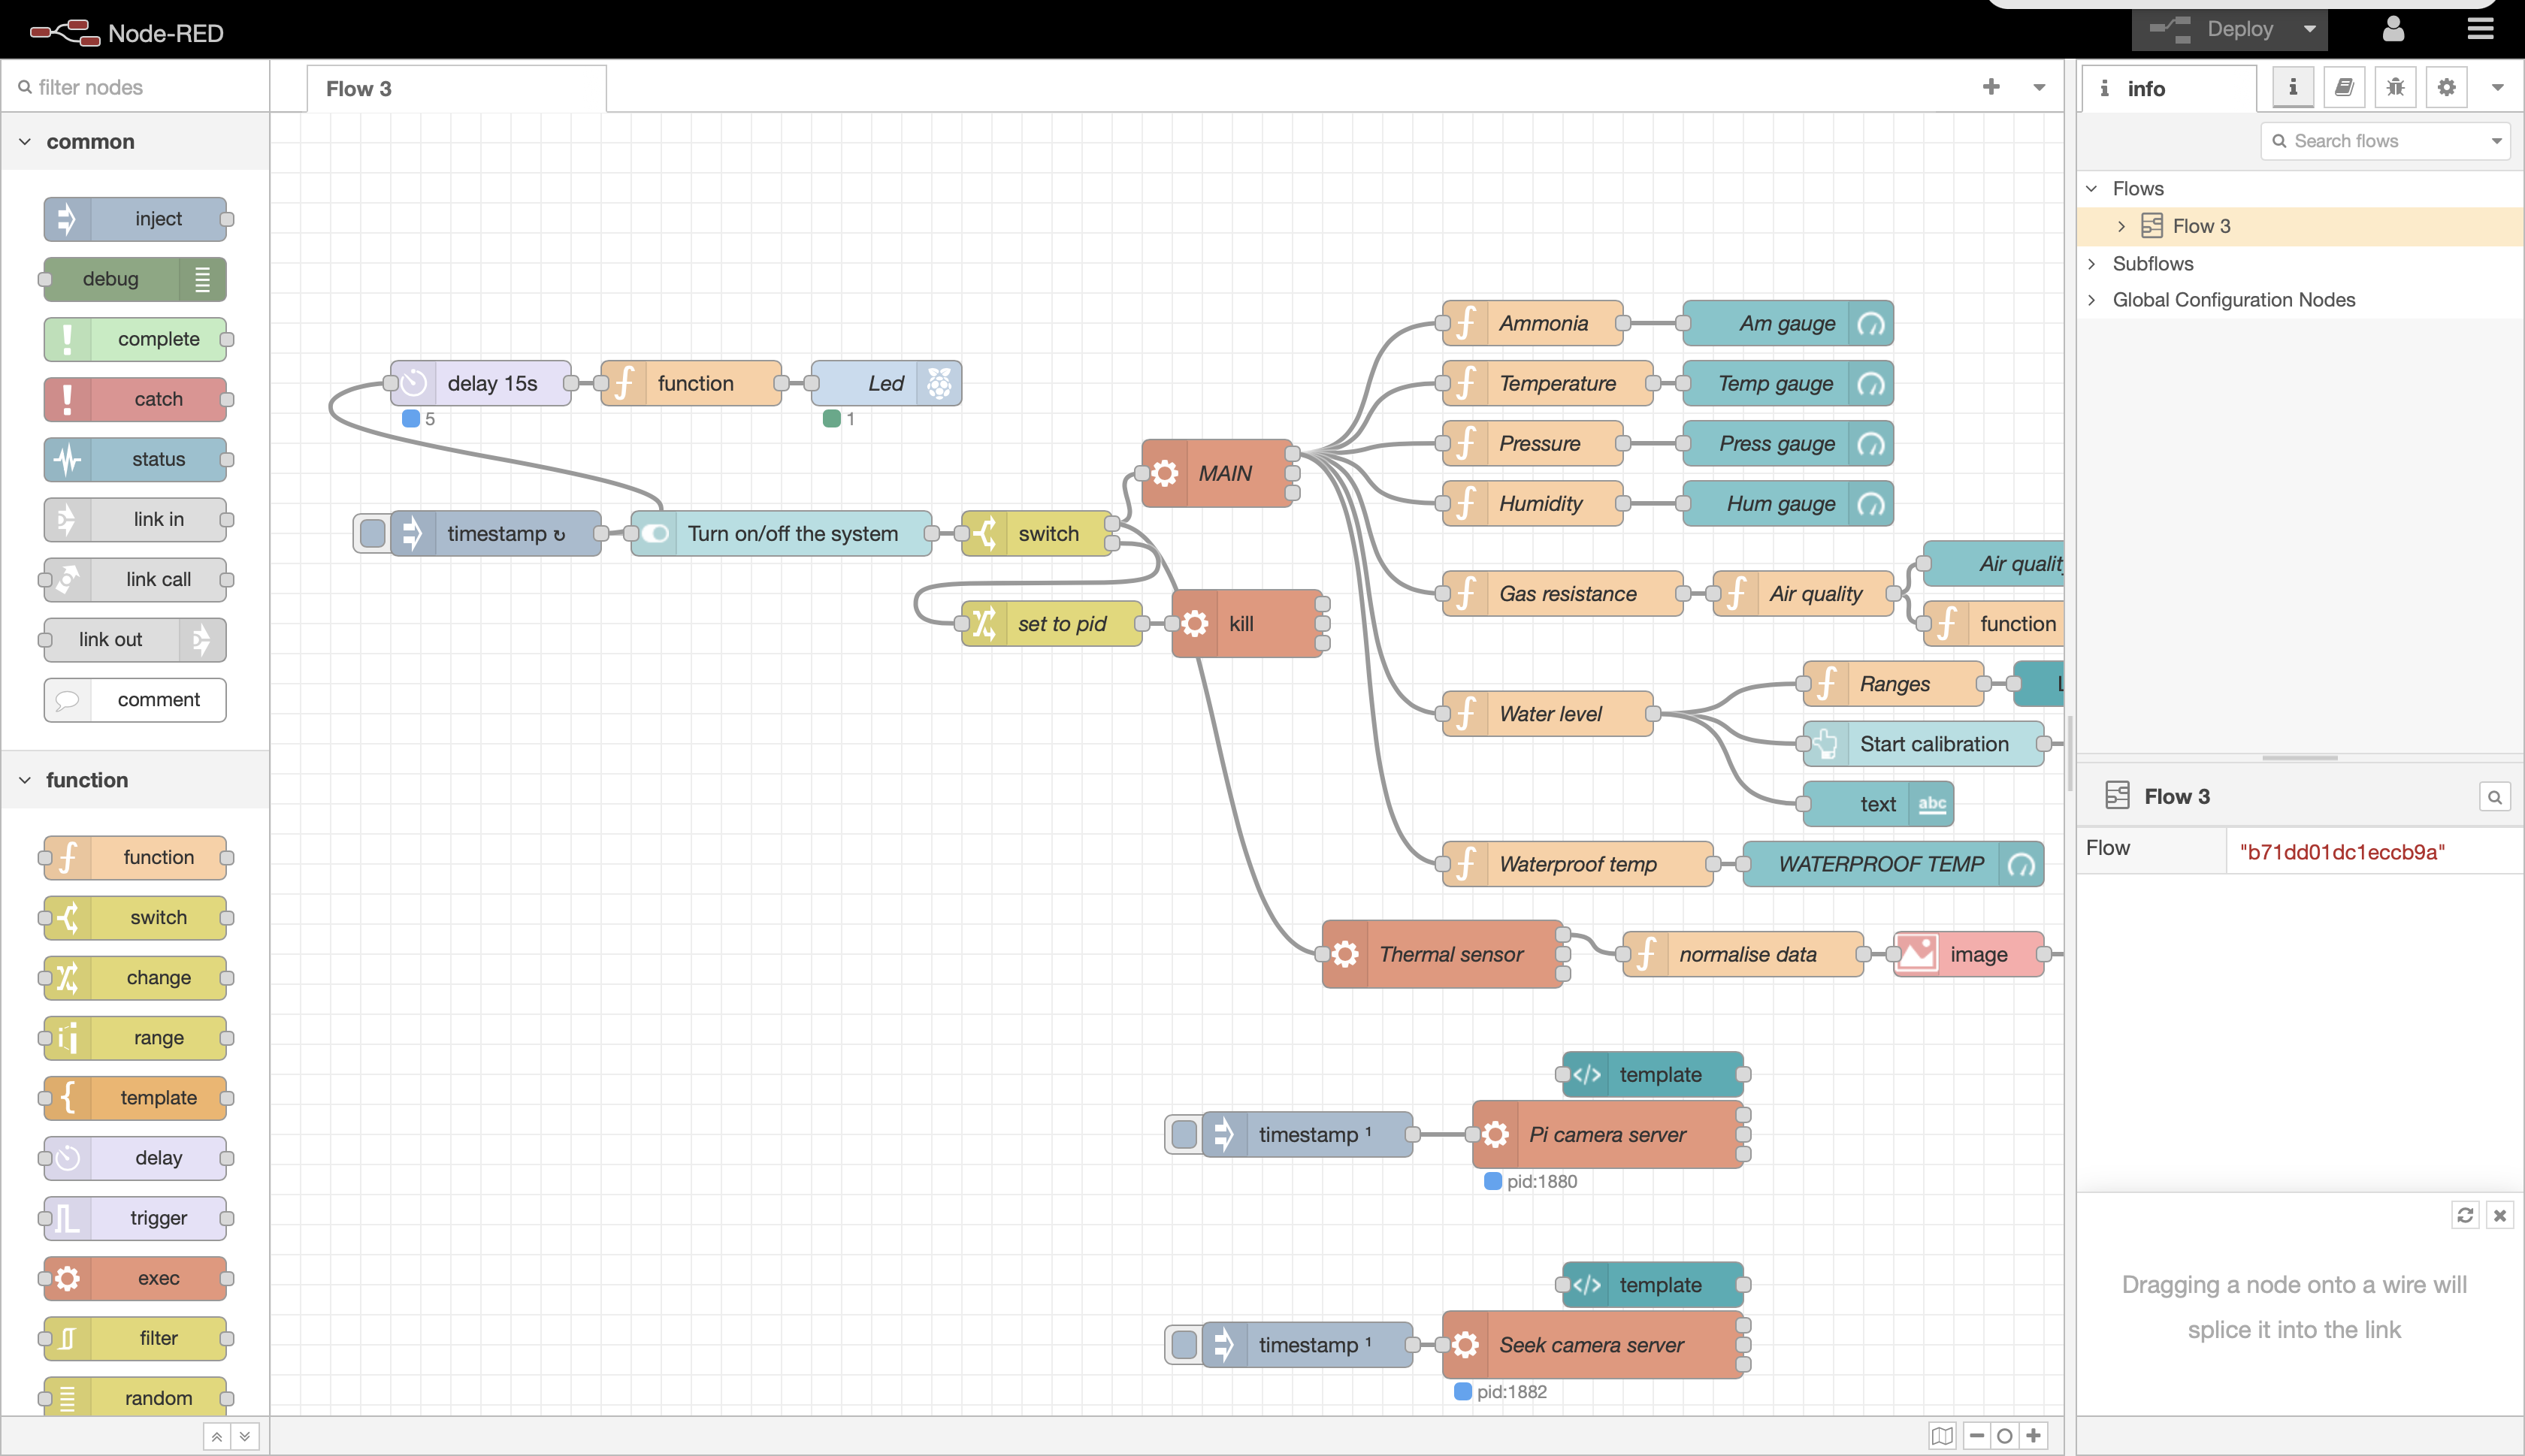
\includegraphics[width=12cm]{figs/nodered-2}}
  \end{center}
\caption{Acceso al flujo de nodos en Node-Red.} \label{fig:adminlogin}
\end{figure}

\begin{figure}[h!]
  \begin{center}
    \subfigure[]{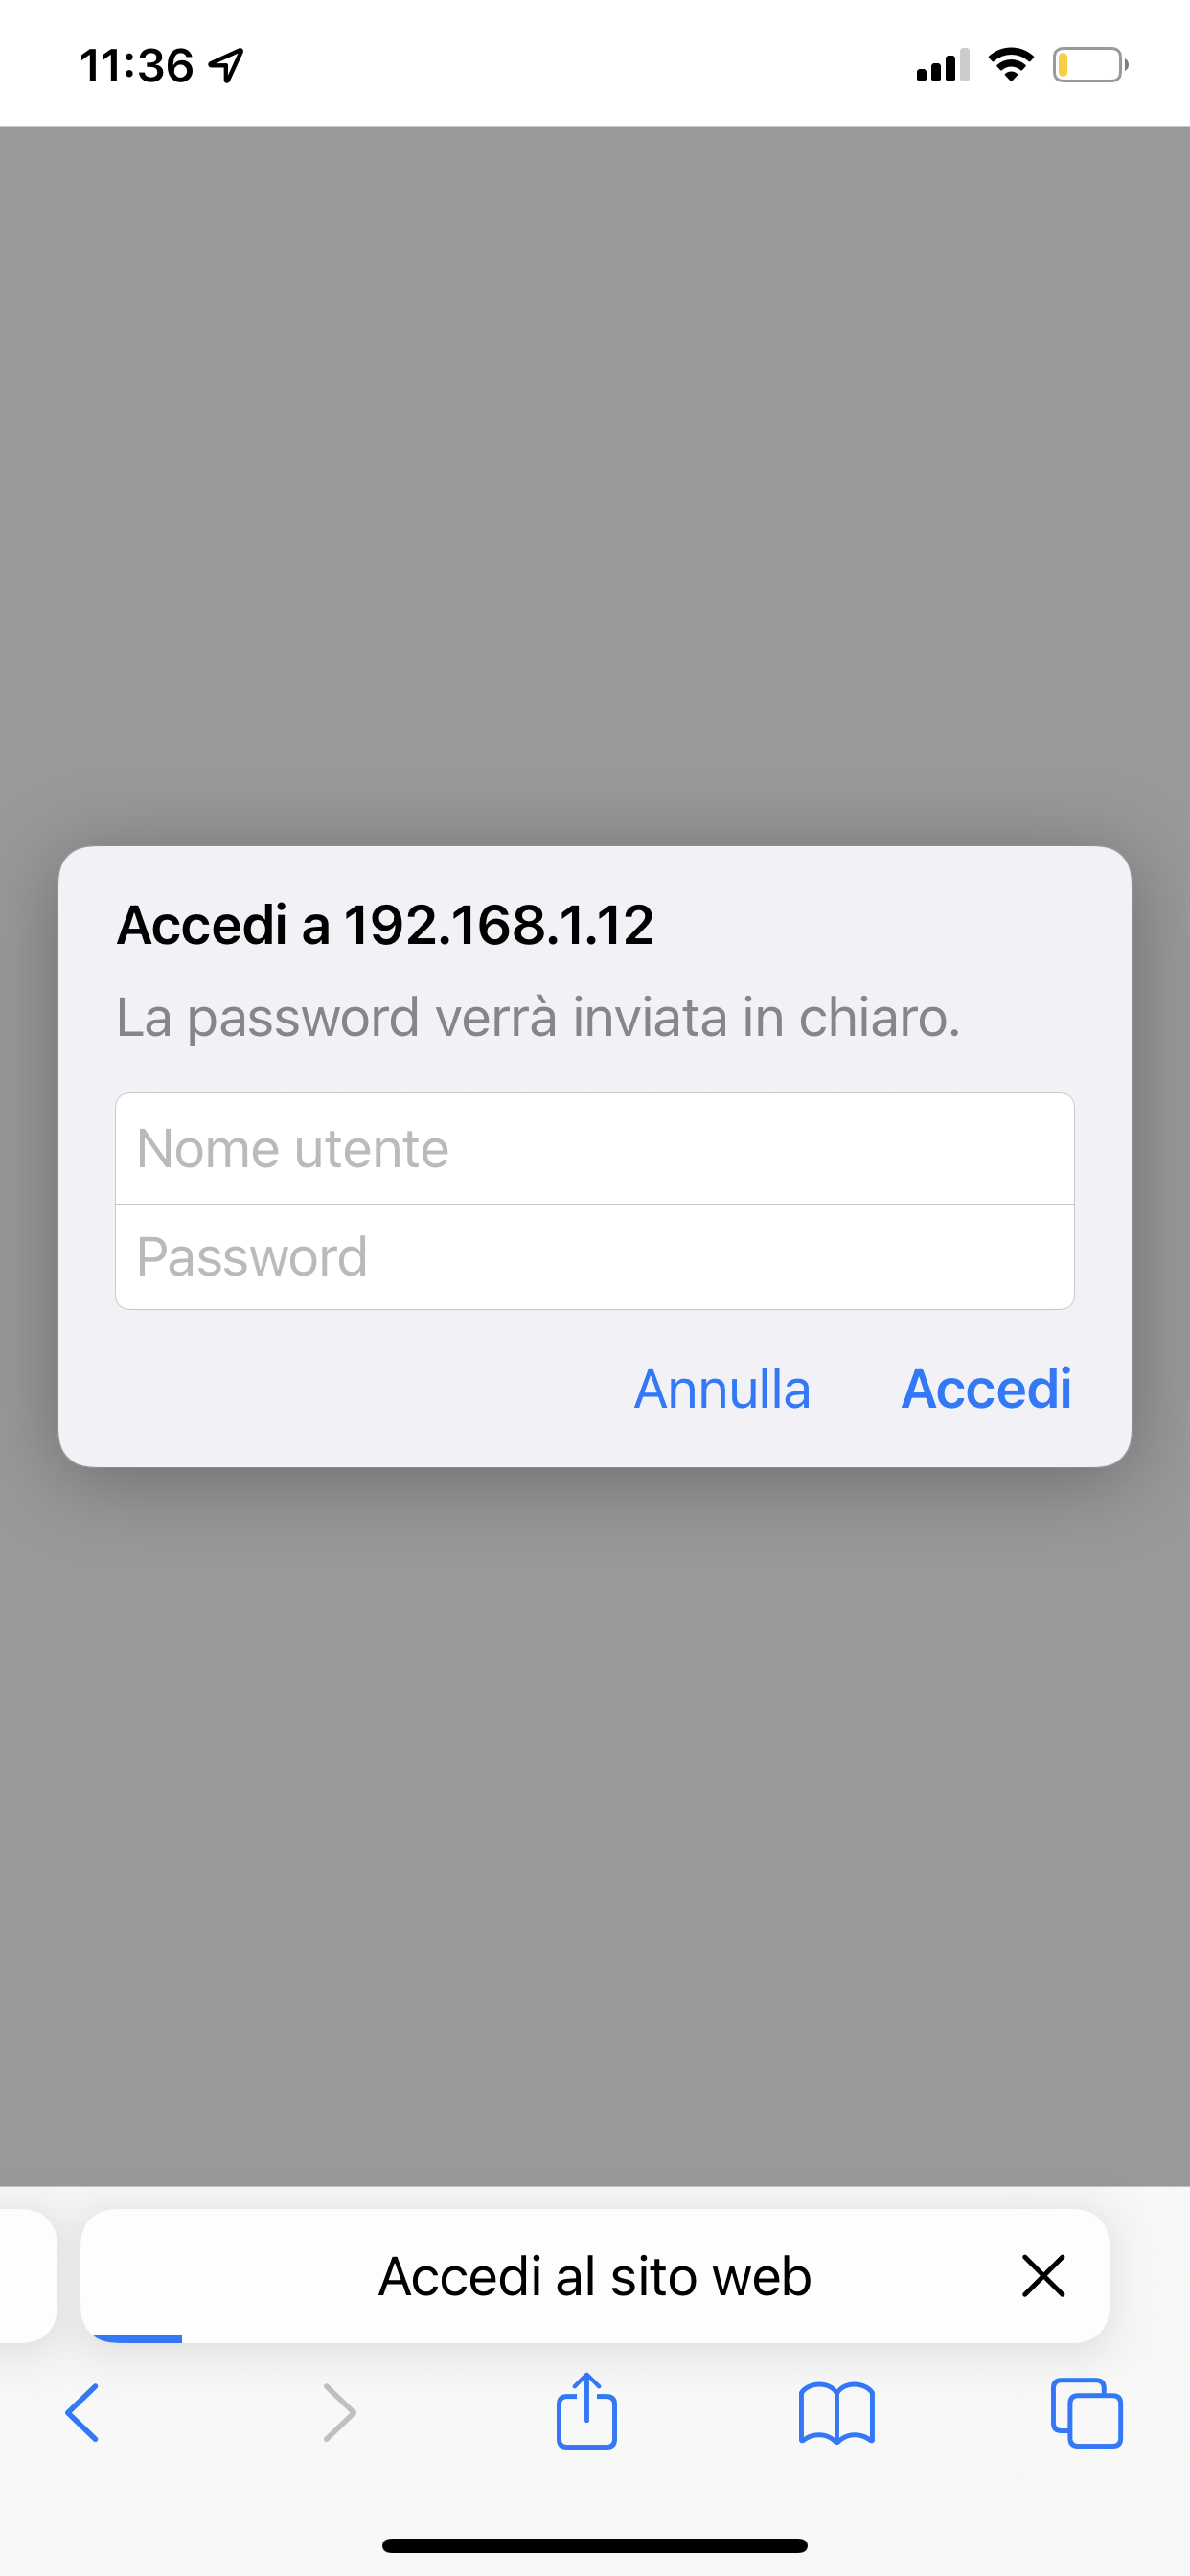
\includegraphics[width=6cm]{figs/phonelogin}}\hspace{2mm}
    \subfigure[]{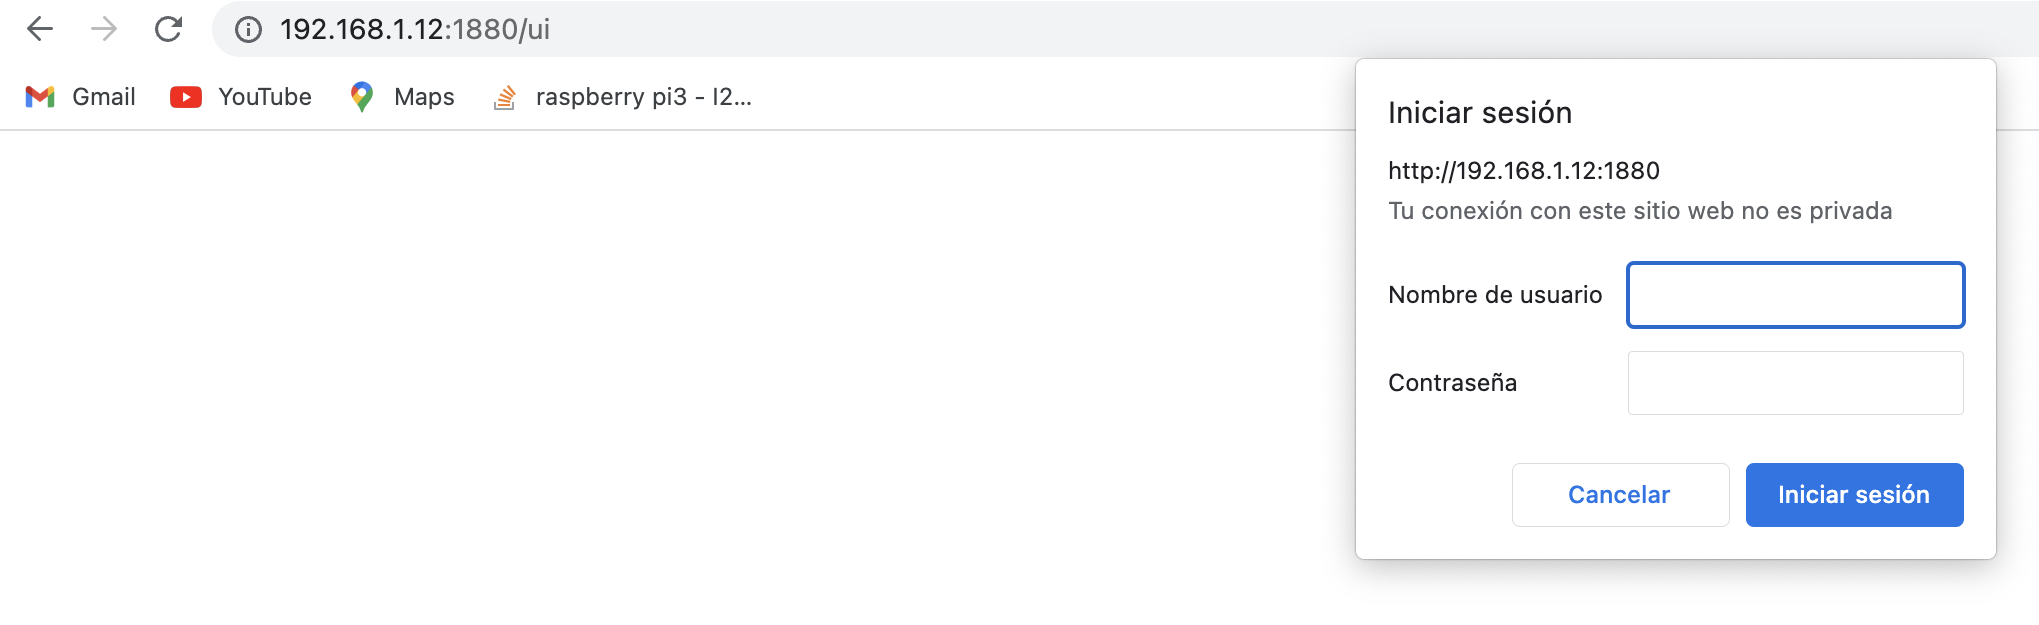
\includegraphics[width=5.5cm]{figs/maclogin}}
  \end{center}
\caption{Acceso a la interfaz de usuario desde distintos dispositivos.} \label{fig:userlogin}
\end{figure}


Por otro lado, tanto los servidores de Flask como Node-Red se lanzan, por defecto, bajo una URL de HTTP (Hypertext Transfer Protocol). Por tanto, un cambio necesario ha sido añadir seguridad, de tal forma que sea HTTPS (Hypertext Transfer Protocol Secure), para impedir que otros usuarios puedan interceptar la información confidencial que se transfiere entre el cliente y los servidores web a través de Internet. Este cambio se ha realizado añadiendo certificados autofirmados creados por el autor.\\

\subsection{Autoarranque}
Recordando que este sistema está pensado para personas que no están familiarizadas con la programación o los ordenadores, se ha considerado añadir una opción que facilite el arranque del sistema.\\

Con el encendido de la Raspberry, la interfaz de usuario se lanza de forma automática ---así como los dos servidores--- y se enciende solicitando el login del usuario para acceder a la IU. Además, se ha incorporado un led verde que se ilumina cuando el sistema está listo para ser usado. El funcionamiento del autoarranque, tanto de Node-Red como de los servidores, se encuentra detallado en la wiki\footnote{\url{https://github.com/jmvega/tfg-icebollada/wiki/5.May-progress}}. El proceso de autoarranque es visible en la Figura \ref{fig:autoarranque}.
\begin{figure}[h!]
  \begin{center}
    \subfigure[Encendido de la Raspberry]{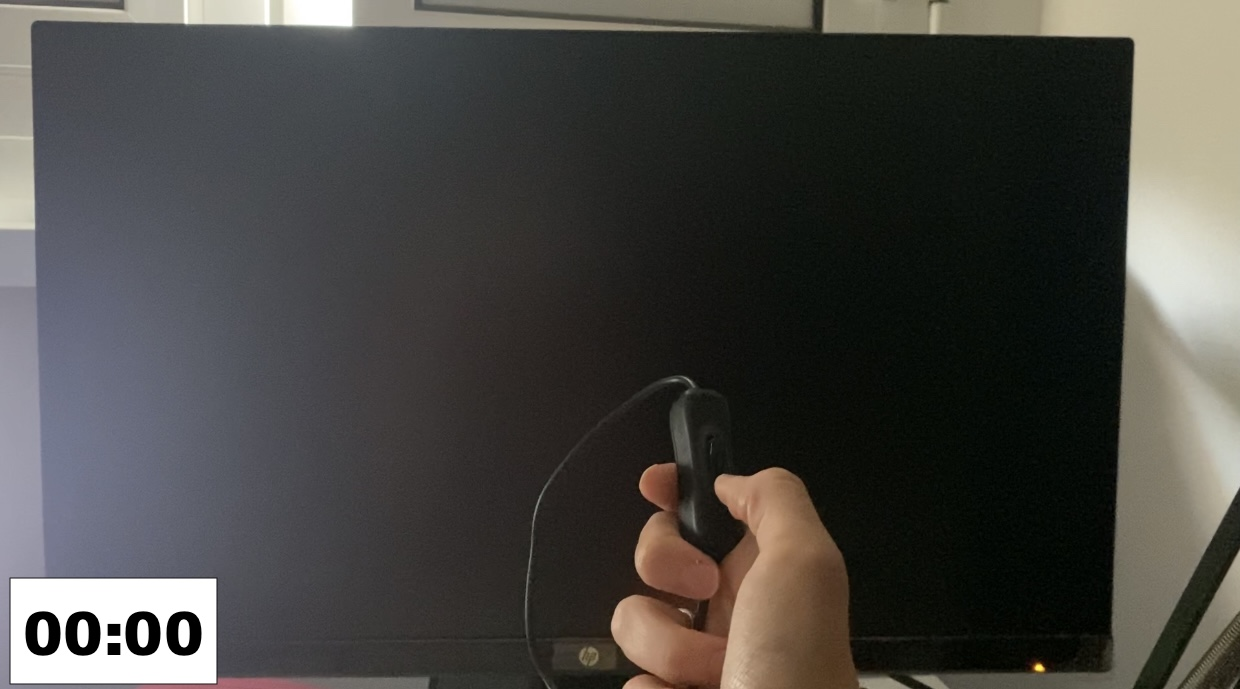
\includegraphics[width=7cm]{figs/auto1}}\hspace{1mm}
    \subfigure[]{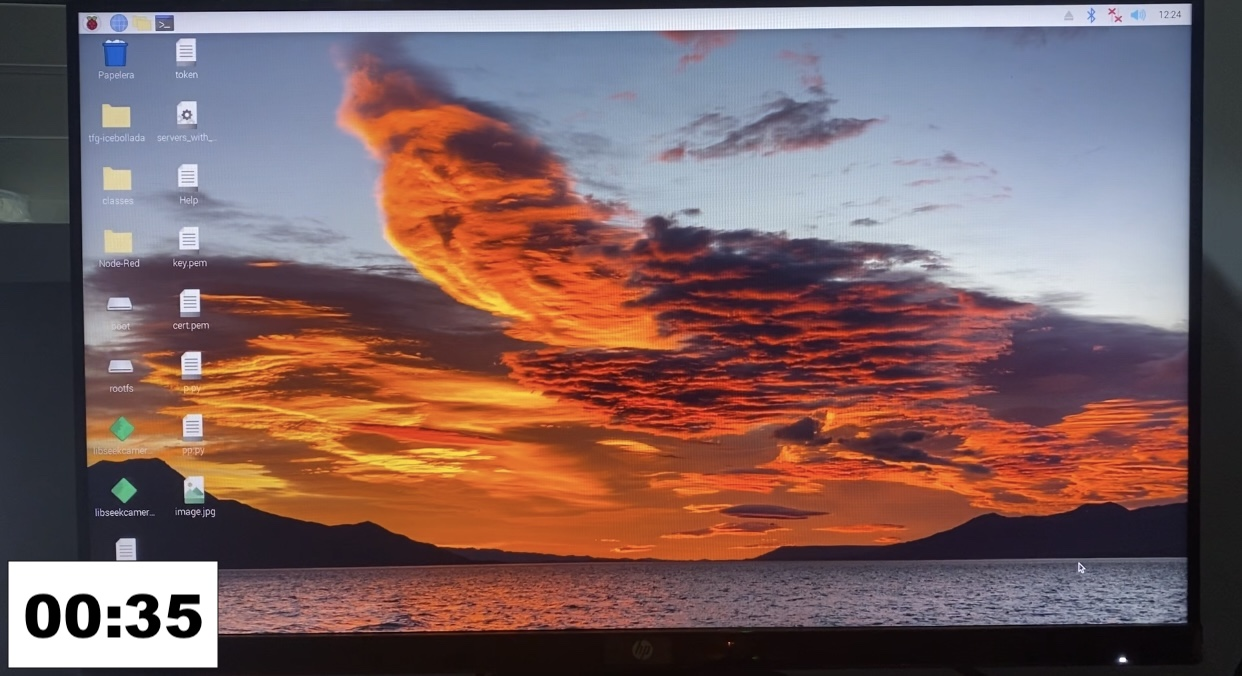
\includegraphics[width=7.2cm]{figs/auto2}}\hspace{1mm}
    \subfigure[]{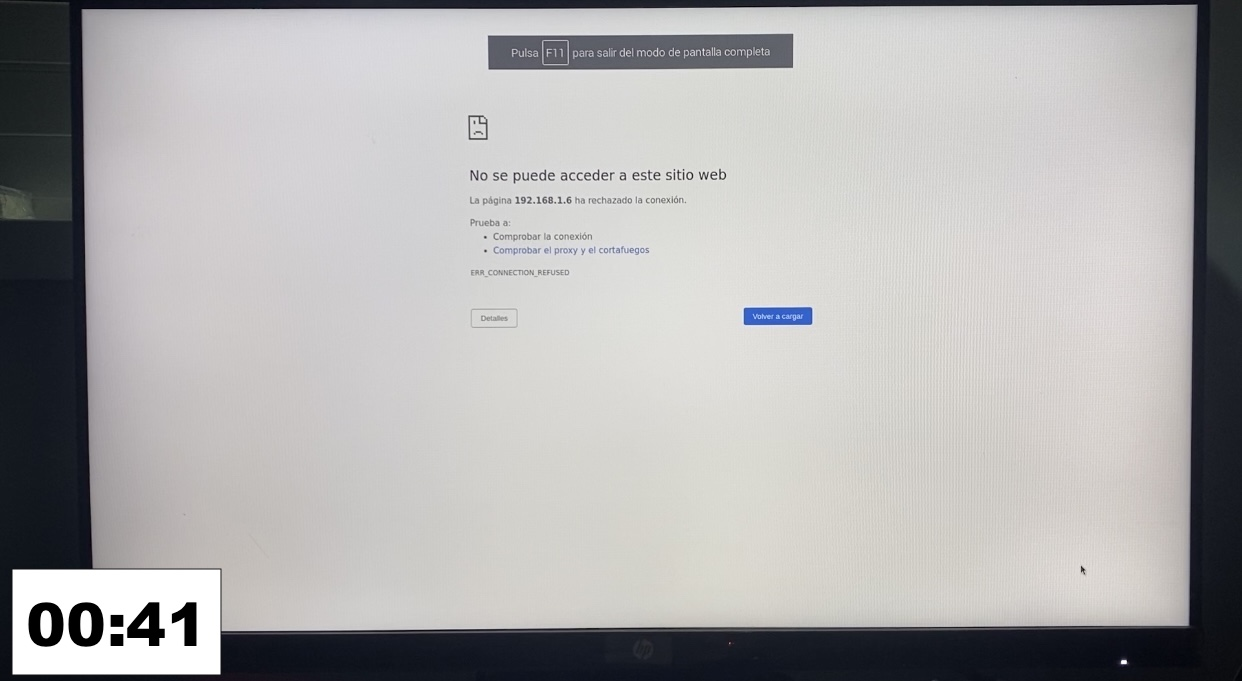
\includegraphics[width=7cm]{figs/auto3}}\hspace{1mm}
    \subfigure[Sistema listo para iniciar sesión]{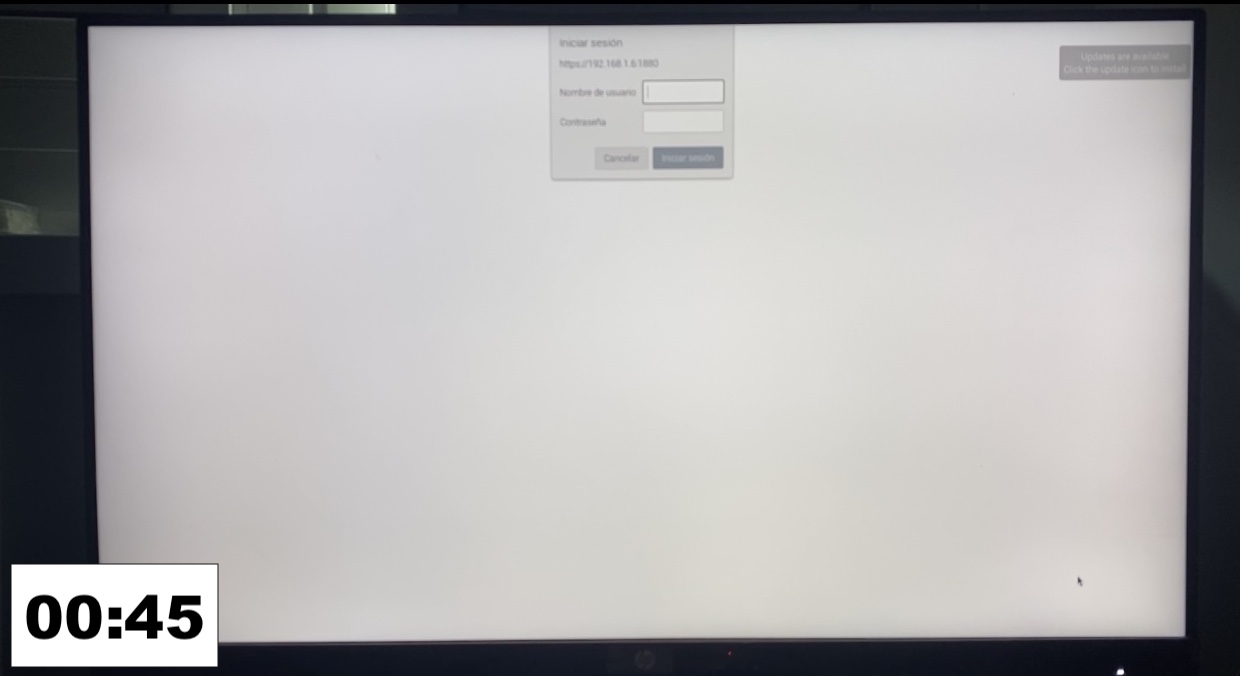
\includegraphics[width=7.1cm]{figs/auto4}}
  \end{center}
\caption{Proceso de autoarranque del sistema.} \label{fig:autoarranque}
\end{figure}

\subsection{Detección de ratones mediante técnicas Deep Learning}
Finalmente, y cumpliendo con el tercer objetivo, se han desarrollado algoritmos para la detección de ratones. Para ello, en primer lugar, ha sido necesaria la creación de un dataset de ratones, debido a que no se ha encontrado ninguno cercano a los objetivos en Internet. Está formado por 354 imágenes: 275 para el proceso de entrenamiento y 79 para el de validación. El dataset creado está disponible en la plataforma Kaggle\footnote{\url{https://www.kaggle.com/datasets/isabelcebollada/datami}}.\\

Una vez se ha obtenido el dataset, se ha procedido a etiquetar estas imágenes mediante la aplicación \textit{labelImg}, para indicar los cuadros limitadores en los que se encuentran los objetos a detectar, en este caso, los ratones. Los ficheros resultantes son .txt compuestos por 5 parámetros: la clase, las coordenadas X e Y mínimas y X e Y máximas de los cuadros delimitadores.\\

Con las imágenes y las etiquetas formadas, se ha procedido al entrenamiento del modelo para la detección de ratones. Esta detección se ha realizado con YOLOv5. YOLO ofrece diferentes modelos que se adaptan a distintas características (Figura \ref{fig:tablayolo}). Se han probado cuatro modelos para la detección de ratones: YOLOv5x, YOLOv5m, YOLOv5s y YOLOv5n, siendo YOLOv5x el más lento pero más preciso y YOLOv5n el más rápido y menos preciso. Debido a que el sistema se utiliza en Raspberry, es importante tener en cuenta que el rendimiento de la CPU es más limitado que en un ordenador normal. Se ha probado el primer modelo (YOLOv5x) en un ordenador normal, donde los resultados han sido muy buenos: La visualización ha sido en tiempo real y la precisión muy buena. Sin embargo, este modelo no ha sido viable en Raspberry debido a la poca velocidad en la que se visualizaban las imágenes. Se ha probado el modelo YOLOv5m, pero el resultado ha sido una velocidad escasa en la placa. También se ha probado con YOLOv5s, donde las imágenes han ido más fluidas, aunque no a tiempo real, pero también la precisión en la detección de ratones ha disminuido. Como última prueba se ha probado con YOLOv5n. La precisión era mucho peor respecto al anterior, y la velocidad era prácticamente igual, por lo que la decisión final ha sido escoger el modelo YOLOv5s. A pesar de que se ha usado uno de los modelos más rápidos, en Raspberry el flujo de imágenes no resulta fluido. Debido a este motivo, la detección no es perfecta; pues hay detecciones incorrectas así como ocasiones en las que no detecta ratones (Figura \ref{fig:detec}). Todos los experimentos realizados pueden encontrarse en la wiki\footnote{\url{https://github.com/jmvega/tfg-icebollada/wiki/6.June-progress}} del proyecto.\\
\begin{figure}[h!]
  \begin{center}
    \subfigure[Detección correcta]{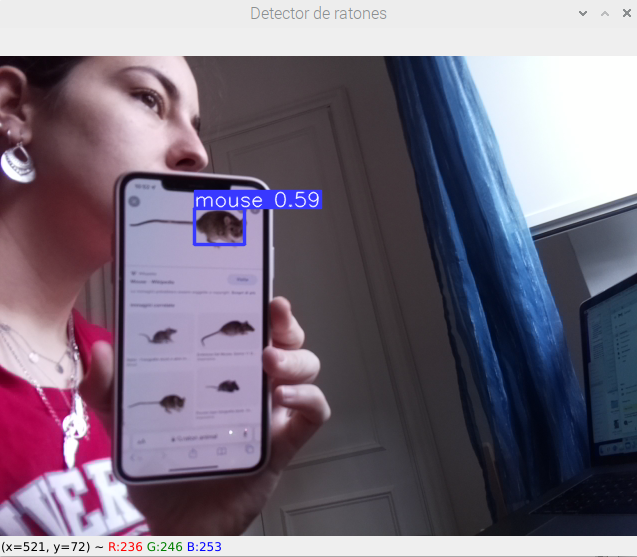
\includegraphics[width=7cm]{figs/correcta}}\hspace{1mm}
    \subfigure[Detección incorrecta]{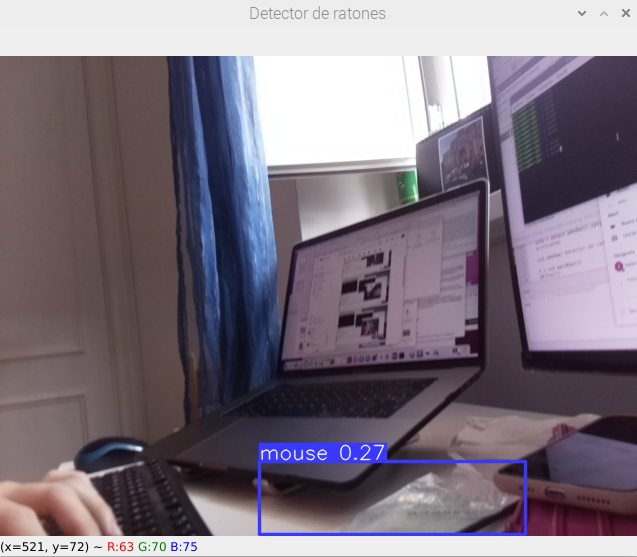
\includegraphics[width=7cm]{figs/incorrecta}}\hspace{1mm}
    \subfigure[No detección incorrecta]{\includegraphics[width=7cm]{figs/nodeteccion}}\hspace{1mm}
    \subfigure[No detección correcta]{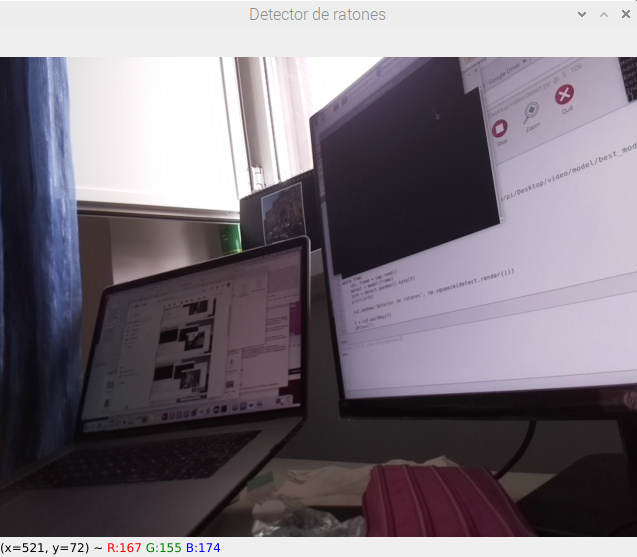
\includegraphics[width=7cm]{figs/nodeteccbien}}
  \end{center}
\caption{Detección de ratones con el modelo entrenado con YOLOv5s.} \label{fig:detec}
\end{figure}

El entrenamiento de YOLOv5 se lleva a cabo a través de un algoritmo de Deep Learning: una red neuronal convolucional. Este utiliza características ya entrenadas proporcionadas por \textit{coco128} ---un dataset muy grande ya existiente--- y aplica el nuevo dataset creado. Después del entrenamiento se obtienen métricas del modelo obtenido (Figura \ref{fig:metricas}), y se puede proceder a la prueba del modelo. En la Figura \ref{fig:precision} pueden verse la predicción de ratones en algunas de las imágenes de validación con el modelo entrenado.\\
\begin{figure}[h!]
  \begin{center}
    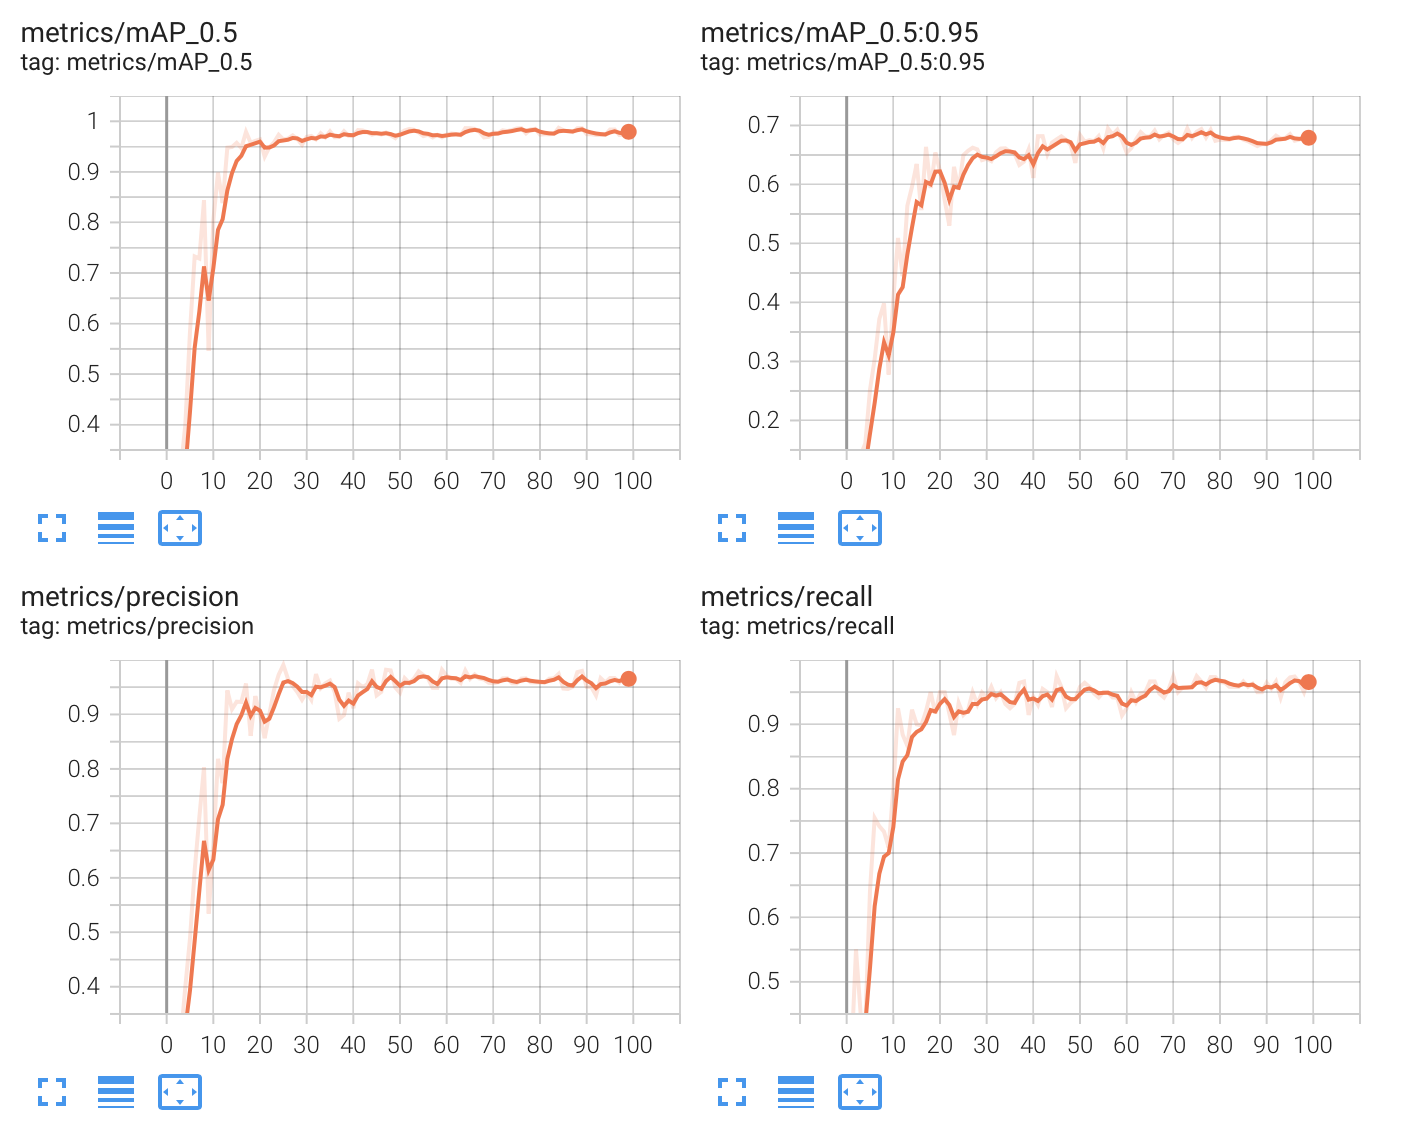
\includegraphics[width=12cm]{figs/metricas}
  \end{center}
\caption{Métricas del modelo entrenado para la detección de ratones.} \label{fig:metricas}
\end{figure}
\begin{figure}[h!]
  \begin{center}
    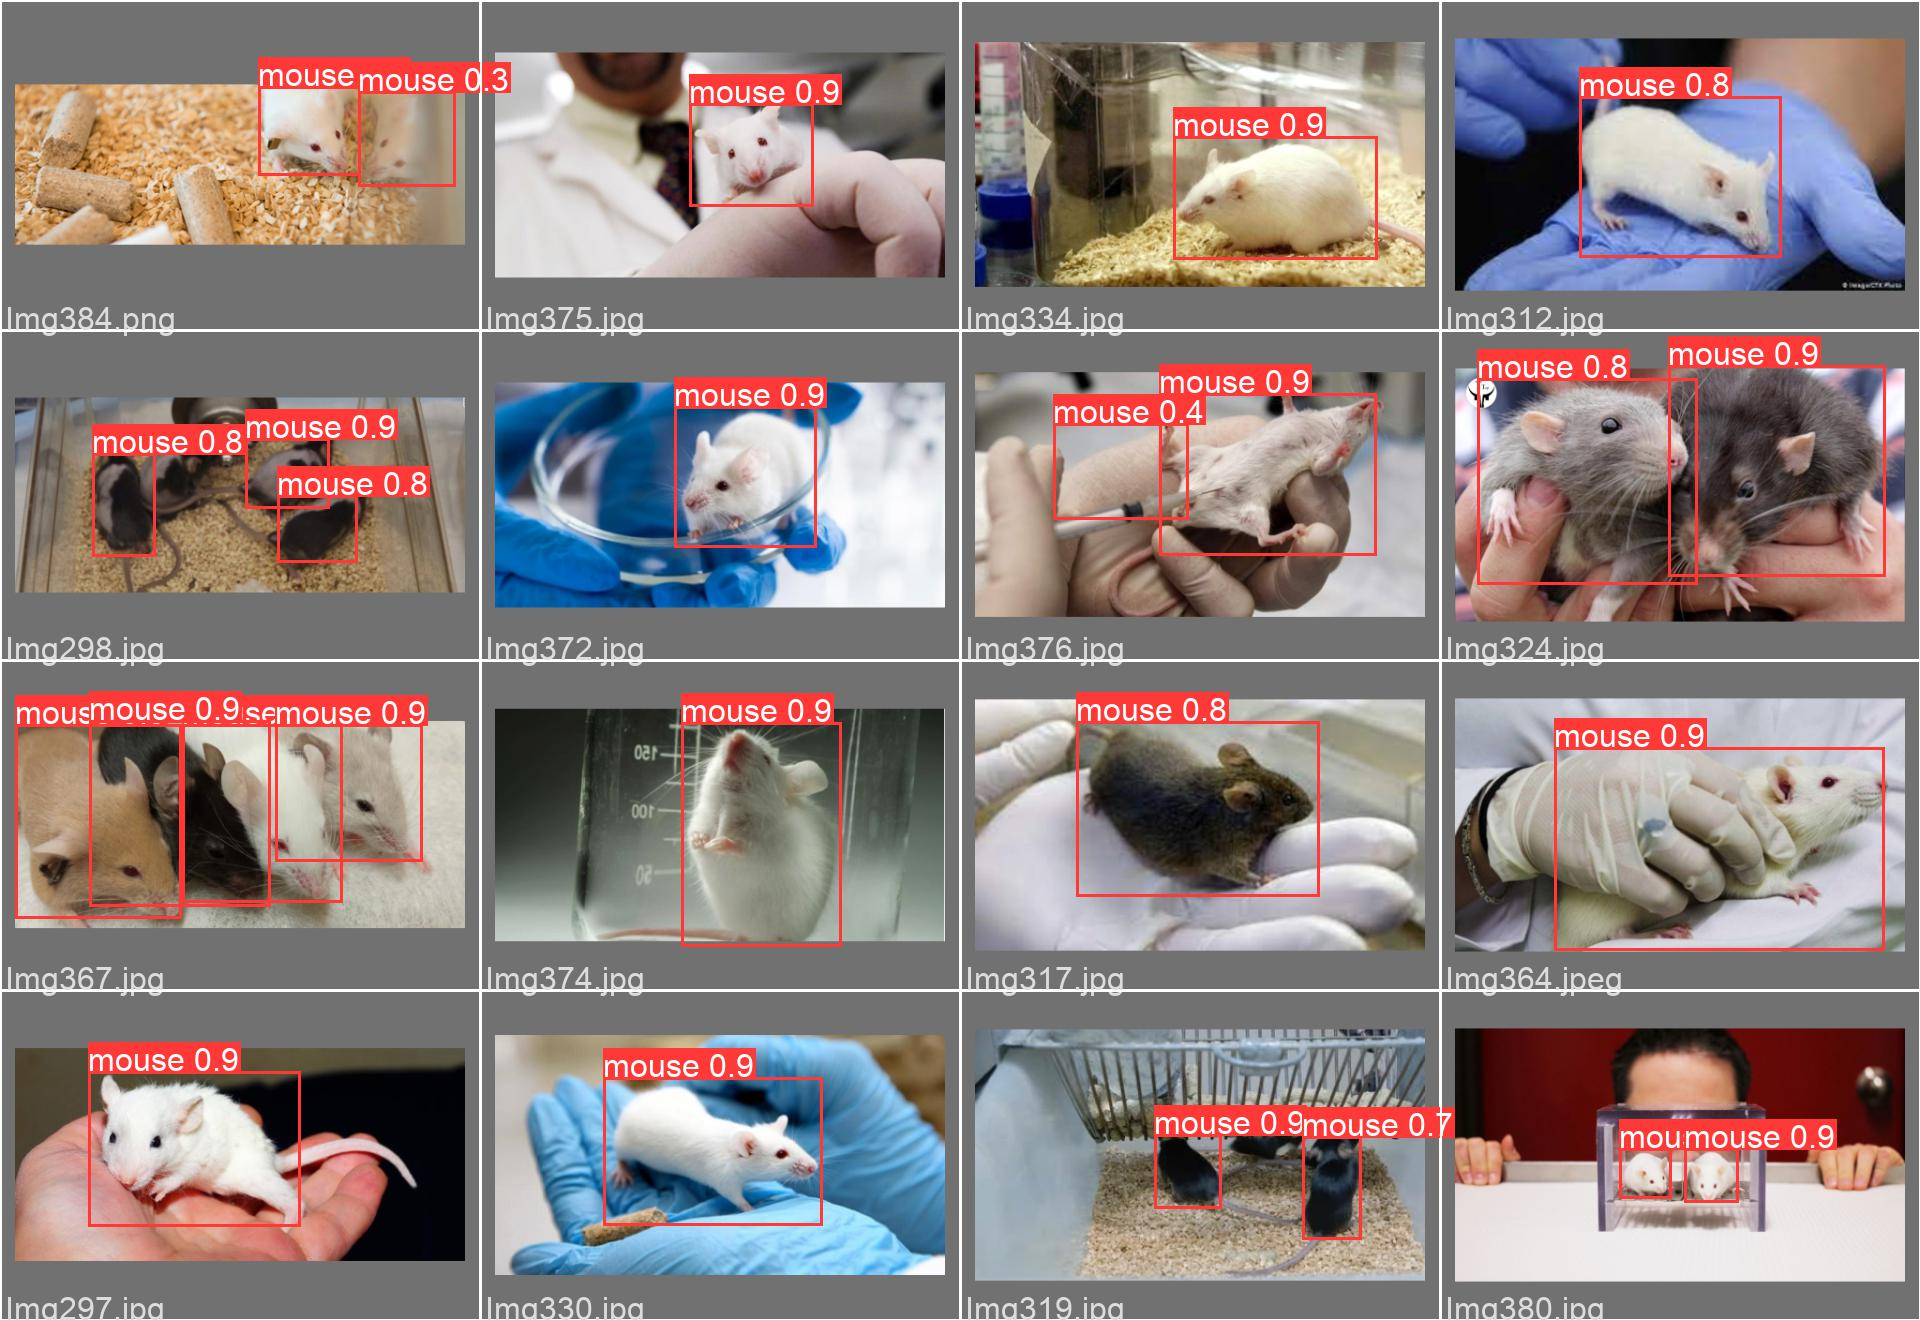
\includegraphics[width=12cm]{figs/precision}
  \end{center}
\caption{Detección de ratones con el modelo entrenado con YOLOv5.} \label{fig:precision}
\end{figure}

Finalmente, con el uso de Python y OpenCV, puede visualizarse la detección de ratones en tiempo real con la PiCamera y la Raspberry. 
